\documentclass[12pt]{article}

\usepackage{amsmath}
\usepackage{graphicx}
\usepackage{caption}
\usepackage{subcaption}
\usepackage{enumerate}
\usepackage{rotating}
\usepackage{multirow}
\usepackage{booktabs}
\usepackage{dcolumn} %for use with R package stargazer
\usepackage[hang,flushmargin]{footmisc} 

\usepackage{setspace}
\usepackage{parskip}
\usepackage[top=1in,bottom=1in,left=1in,right=1in]{geometry}

\usepackage[utf8]{inputenc}

\usepackage{natbib}

\usepackage{hyperref}
\hypersetup{pdfstartpage=1, pdfpagemode=UseNone, pdfstartview=FitH, pdffitwindow=true, bookmarks=false, colorlinks=true, linkcolor=blue, citecolor=blue}

\title{Temporary employment in Europe: Stagnating rates and rising risks}

\author{Jonathan P. Latner\thanks{Universit{\"a}t Bamberg} \footnote{\url{jonathan.latner@uni-bamberg.de}.  This project has received funding from the European Research Council (ERC) under the Horizon 2020 research and innovation program (grant agreement No 758491).  The author would like to thank the following individuals (in alphabetical order):  Sophia Fauser, Michael Gebel, Chen-Hao Hsu, Andreas Haupt, Richard Latner, Ellen Pechman, Klaus Pforr, James Raymo, Sonja Scheuring, Jody Schimek, attendees of the CSIS Brown Bag Seminar at the University of Trento, and the reviewers and editors of European Societies.  Replication files are located here:  \url{https://doi.org/10.7910/DVN/ZBLXPR}}}

\date{\vspace{-5ex}}

\newcommand\wordcounttot{\input{word_count_tot.sum}} 

\begin{document}

\maketitle

\begin{abstract}

\noindent 
There is a perception that temporary employment is rising in Europe, but there is little evidence to support this.  If one takes the position that temporary employment should be rising due to large structural changes in European labour markets, then stagnating trends represents something of a puzzle.  I examine the puzzle by applying a life course approach to understand the distribution and trends in temporary employment among prime age workers in 31 European countries.  I compare and contrast changes in the temporary employment rate in a single period of time using cross-sectional data from the European Labour Force Survey (LFS), with changes in the risk of experiencing temporary employment in multiple periods of time using longitudinal data from the European Survey of Income and Living Conditions (SILC).  Results from cross-sectional data suggests that between 1996 and 2007, the temporary employment rate increased in Europe by 28\%, but between 2007 and 2019, there was little change.  By contrast, results from panel data suggests that between 2013 and 2019, the risk of experiencing at least one temporary employment contract rose 36\%.  Over time, the temporary employment rate stagnated, but the temporary employment risk rose.  The contribution provides insight into the nature of employment experiences associated with insecurity.  

\noindent
\\
{\bf Key words:} temporary employment, trends and distribution, life course, international comparison, labour markets, Europe \\
{\bf JEL Classifications:} Z13 (economic sociology, economic anthropology, social and economic stratification), J21 (labour force and employment, size, and structure), J08 (labour economics policies)

% \noindent
% \\
% {\bf Total word count (including these words):} \wordcounttot

\noindent
\\
{\bf Revision date:} \today

\noindent
\\
{\bf Authors note:} This article has been accepted for publication by, \emph{European Societies}.  
% This draft is not for (re)distribution or citation without the permission of the author.
\end{abstract}

\clearpage
\section{Introduction}
\doublespacing

It is often stated that temporary employment is rising in Europe \citep{ter_weel_2018,biegert_kuhhirt_2018,hogberg_etal_2019,crouch_2019,reichenberg_berglund_2019}.  And with good reason.  The expectation is that temporary employment should be rising due to a profound restructuring of European labour markets since the 1970s \citep{esping-anderson_regini_2000}.  A primary reason was that in the 1970s and 1980s, high levels of unemployment and low levels of economic growth characterized many European economies \citep{giersch_1985}.  Compared to the United States, many feared that Europe was falling behind \citep{oecd_2003}.  To address the problem, the Organization for Economic Co-operation and Development (OECD) recommended policy changes to make labour markets more flexible \citeyearpar{oecd_1994,oecd_1996}.  Most countries implemented some variation of the recommendations.  Since then, labour market performance improved \citep[pg. 7]{oecd_2006}, but employment also became less standardized \citep{barbieri_2009}.  

However, since 2000, there is little change in the incidence and distribution of nonstandard work in Europe, a point that others also make \citep{bernhardt_2014,pyoria_ojala_2016,lewchuk_2017}.  There are two main types of nonstandard employment relations, involuntary part-time work and temporary employment \citep{kalleberg_2018}.  According to OECD.Stat, average levels of involuntary, part-time work are rising, but levels are low, from 3\% in 2000 to 5\% in 2018.  In contrast, average levels of temporary employment are much higher, but remained virtually unchanged, from 13\% in 2000 to 14\% in 2018.  I focus on temporary employment not only because it is a more prominent form of nonstandard work, but also because it is not rising, despite expectations to the contrary.  Further, even though there are large differences in levels of temporary employment between countries and demographic groups, there is little change over time within countries and demographic groups \citep[ch. 4]{gebel_giesecke_2009,allmendinger_etal_2013,eurofound_2015,oecd_2015}.  

If one takes the position that temporary employment should be rising due to large structural changes in European labour markets, then stagnating trends represents something of a puzzle.  One possibility is that temporary employment is not rising because other large social forces counteract the structural reasons that otherwise predict a higher incidence of temporary work.  For example, in Europe, technological change increases employment growth at the top of the skill spectrum and decreases it at the bottom \citep{oesch_piccitto_2019}.  The problem is that temporary employment is concentrated at the bottom of the skills spectrum \citep{gebel_giesecke_2016}, where employment is declining.  The point is that there are good reasons to expect little change in the incidence of temporary work.

An alternative explanation is that temporary employment is rising, but the data may underestimate both the size and growth \citep{howell_kalleberg_2019}.  I examine the puzzle by applying a life course approach to understand the distribution and trends in temporary employment in Europe among prime age workers.  Distinct from previous research, I use both cross-sectional data from the European Labor Force Survey (EU-LFS), which surveys different individuals in different time periods, and panel data from the European Survey of Income and Living Conditions (EU-SILC), which surveys the same individuals in different time periods.  In so doing, I distinguish between the temporary employment rate in one time period from temporary employment risk in multiple time periods and distinguish between the risk of experiencing temporary employment from the frequency or duration of temporary contracts (i.e. `spells').  

The result is a more complete accounting of trends and the distribution of temporary employment.  Cross-sectional data suggests that between 1996 and 2007, the temporary employment rate increased in Europe by 28\%, as well as within most countries and demographic groups, but between 2007 and 2019, the temporary employment rate remained virtually unchanged.  Therefore, general claims about rising temporary employment rates in Europe are outdated unless one is referring to specific countries, demographic groups, or time periods.  

By contrast, panel data suggests that the temporary employment risk is not only much higher than the rate, but is also rising, especially after 2013.  Since the 2013 panel wave, the risk of experiencing at least one temporary employment contract rose 36\%.  At the same time, there was little change in the distribution of rising risk between demographic groups or countries.  Further, the risk of receiving a multi-year contract is rising and the risk of receiving multiple contracts is constant or declining.  Together, the interpretation is that the relative insecurity of temporary employment may be declining even as the risk of experiencing a temporary contract is rising.

Comparing and contrasting results from two different data types reveals something about the nature of employment insecurity associated with temporary employment that is not otherwise understood if one uses only cross- sectional or panel data.  Here, insecurity is objectively defined as employment insecurity, as measured by contract type.  Relative to permanent contracts, temporary contracts not only have lower levels of employment security and stability, by definition of the contract itself, but also offer lower average wages and benefits \citep[ch. 4]{eurofund_2015}.  

The temporary employment risk in Europe is more than double that of the temporary employment rate. Therefore, the experience of employment insecurity is much more common that would otherwise be understood to be true if one only focused on the temporary employment rate. Further, unlike the temporary employment rate, the temporary employment risk is rising. Therefore, the evidence suggests that increasing labour market flexibility did come at the cost of rising employment insecurity, but in a way not yet quantified. The nature of employment insecurity that is captured by the temporary employment rate is not rising. Instead, it is the temporary employment risk that is rising.

\section{Background}

\emph{Arguments for rising temporary employment}

Previous literature offers three broad approaches for explaining differences and change in temporary employment levels and trends: welfare regime typology, precariousness, and dualization \citep{hipp_etal_2015}.  In Europe, levels of temporary work have long been understood to be affected by labour market institutions, especially the rules and regulations that govern collective bargaining agreements between employers and unions as well as employment protection \citep{giesecke_gross_2004}.  Differences between countries in their labour market institutions are often categorized into a typology of welfare regimes that are correlated with country-clusters \citep{esping-anderson_regini_2000}, Liberal (Anglophone), Mediterranean (Southern), Conservative (Continental), Social Democratic (Nordic), and Post-communist (Eastern) \citep{van_lancker_2012}.  While far from perfect, the typology captures the general idea that levels of temporary employment are lower in Anglophone countries and higher in Southern countries, with Continental, Nordic and Eastern European countries somewhere between those extremes, owing to differences in labour market regulation.  

The literature on precariousness emphasizes change over time in levels of insecurity captured by nonstandard work arrangements.  Work became more precarious because of a decades-long shift from the coordinated market economy to the liberal market economy \citep{thelen_2014}.  In the first half of the 20th century, the labour market was divided into a primary and secondary segment, which was distinguished by job quality.  Employers relied on the primary segment to meet long-term demand for labour and the secondary segment to meet their short-term demand for labour.  Beginning in the 1970s, owing in part to a series of economic crises, new thinking emerged \citep{oecd_1986}.  Labour market segmentation discouraged employers from hiring new employees, even in times of economic prosperity, owing to the challenge of firing employees in times of economic decline or change \citep{lazear_1990}.  

Increasing economic growth required a new solution.  In the 1990s, the OECD released \emph{The Jobs Study} \citeyearpar{oecd_1994} and \emph{The Jobs Strategy} \citeyearpar{oecd_1996}.  These reports included nine policy recommendations, all of which were designed to reduce labour market segmentation and increase labour market flexibility.  The problem is that adopting American style, pro-competitive reforms decreased unemployment and increased labour force participation, but other elements were imported as well, like the job insecurity that comes with employment-at-will, as approximated by the European use of temporary contracts \citep{oecd_2006}.  This implies a trade-off between flexibility and employment security \citep{muffels_2014}.  As evidence, since 2000, temporary employment accounts for the majority of new job growth \citep[Fig. 6]{eurofound_2015}.  Therefore, the expectation is that levels of temporary employment are rising. 

The literature on dualization emphasizes the growing compositional differences between regular and nonstandard jobs \citep{emmenegger_etal_2012}.  The primary and secondary segments described above were not equally distributed across population groups with primary segments dominated by prime-aged, educated, men.  As labour markets became more flexible and labour force participation rates rose, the composition of the workforce also changed, especially with respect to age and gender.  Dualization describes the process of protecting the primary segment from the consequences of providing employers with more flexibility, and exposing the secondary segment, especially women \citep{gash_mcginnity_2007}, younger workers \citep{allmendinger_etal_2013}, and those with less education \citep{gebel_giesecke_2009}.  This process is also referred to as `recommodification of risks' \citep{breen_1997}.  Therefore, the expectation is that rising levels of temporary employment are distributed unequally across the population, and concentrated in more vulnerable groups. 

\emph{Arguments against rising temporary employment}

There are two main arguments against the idea that temporary employment should be rising.  One emphasizes the role of technological change on the demand for labour by skill.  In most European countries, workers with low levels of education face the highest relative risk of holding a temporary contract \citep{gebel_giesecke_2016}.  While employment polarization by skill characterizes the more liberal labour markets in America and the United Kingdom, institutions in the more regulated European continental countries channel technological change into various patterns of upgrading, with increases at the top of the skill spectrum and declines at the bottom \citep{oesch_piccitto_2019}.  Therefore, one should not expect temporary employment to be rising at the population level if employment is rising in high-skill occupations, where temporary employment is not dominant, and declining in low-skill occupations, where temporary employment is dominant.

Another plausible mechanism emphasizes the role of educational expansion.  The job security that comes with a permanent contract is a valuable asset, which some workers may be willing to trade \citep{ortiz_mcguiness_2018}.  Developments towards a higher educated population give labour supply more power to secure a better job match.  The assumption is that job match refers to skills match, but other preferences also exist.  Some may prefer to trade higher education for more job security, albeit at the cost of skills match, i.e. over education.  As evidence, over education is more likely in permanent employment, especially in segmented labour markets where a permanent contract is more valuable \citep{ortiz_2010}.  Therefore, rising levels of education may offset rising levels of temporary employment at the population level.  The broader point is that there are good reasons to expect little change in the incidence of temporary work.

\emph{A life course approach}

An alternative explanation is that temporary employment is rising, but is hidden in the data.  Previous research on temporary employment trends in Europe used cross-sectional data.  The problem is that cross-sectional data can only capture the prevalence of temporary employment in a single period of time, i.e. the temporary employment rate.  By contrast, panel data captures the risk of experiencing temporary employment in multiple periods of time.  To understand the difference, I borrow classic concepts from the life course approach to understand the role of time in how individuals experience events \citep{mayer_tuma_1990}.

One concept is that the proportion of people who experience an event in multiple periods of time is often higher than the proportion who experience that same event in a single period of time.  This concept is referred to as `heightened risk.'  Distinguishing one from the other explains why the temporary employment rate can remain stagnant, but the risk of temporary employment can rise.  The reason is that a very small up-and-down change in the year-to-year temporary employment rate can result in a rising risk of temporary employment when the small change is multiplied over time.

To illustrate the idea of heightened risks, let us imagine a simple economy with three people in two panel periods ($A$ and $B$), each of which are 3 years long.  In panel period $A$, in each year, 1 person had a temporary employment contract and 2 people had a permanent employment contract.  The temporary employment rate in each year is 0.33.  Further, the same person had a temporary employment contract in each period.  Therefore, in panel period $A$, the risk of experiencing temporary employment is 0.33, because one person experienced temporary employment, and two people never experienced temporary employment.  

As in panel $A$, in panel $B$, in each year, 1 person had a temporary employment contract and 2 people had a permanent employment contract.  The temporary employment rate in each year remains the same 0.33.  However, unlike panel $A$, in panel $B$, the same person had a temporary contract in the first two periods, but a different person had a temporary contract in the third period.  Therefore, in panel $B$, the temporary employment risk is 0.66, because two people experienced temporary employment and one person did not.  The example illustrates how the risk can rise, even if the rate does not.

A second concept is that one must distinguish the probability of experiencing an event from the frequency or duration of that event.  These are referred to as `spells,' and inform our understanding about whether insecurity is changing within temporary employment contracts.  

Multiple, sequential contracts are more insecure than a single contract.  The reason is that, relative to a single temporary contract, research has long shown that the consequences of multiple temporary contracts negatively affects wages and career mobility outcomes \citep{booth_etal_2002,mertens_mcginnity_2004}.  The theoretical explanation is that temporary employment can sometimes, but not always act as a `trap' that reduces opportunity for mobility, with cycles of repeated temporary jobs, short permanent jobs, and unemployment  \citep{fuller_stecy-hildebrandt_2015}.  

At the same time, with respect to duration, a temporary contract that is multiple years long is more secure than a temporary contract that is one year long or less, by definition of the contract length. Further, some evidence suggests that the longer the duration of the temporary contract, the higher the likelihood of moving from a temporary to permanent contract \citep{gagliarducci_2005}.

A third concept in life course research addresses stratification.  Temporary employment is a life event, and, like other life events, the risk of experiencing that event is not distributed equally between groups.  With respect to temporary employment, important characteristics are age \citep{hipp_etal_2015}, gender \citep{gash_mcginnity_2007}, and education \citep{gebel_giesecke_2016}.  Research has long established inequalities in the risk of temporary employment by these demographic groups.  However, research has not yet examined changes over time by demographic groups in the risk of temporary employment, by itself, or the number and duration of temporary contracts.  Such inequalities in the stratification of risk over time are crucial to understand whether changes in risk are distributed equally or, for example, if rising risk is concentrated among already vulnerable groups.

In summary, a life course approach includes several key concepts to better understand trends in the level and distribution of temporary employment: rate, risk, frequency, duration, and stratification.  While previous research applied the life course approach to examine divorce \citep{kennedy_ruggles_2014}, poverty \citep{sandoval_etal_2009}, unemployment \citep{dietrich_2013}, etc., I am not aware of a similar application to temporary employment trends and distribution.  A key contribution of our paper is that the analysis integrates all these key elements in our analysis.

\section{Data}

Two types of data are required to examine trends in temporary employment over time using a life coarse approach.  First, most importantly, one needs panel data.  Panel data are used to analyze the risk of experiencing a temporary employment contract, as well as the duration and number of contracts in multiple periods of time.  Second, one needs cross-sectional data.  Cross-sectional data are used to analyze the rate, or the prevalence of temporary employment in a single period of time.  Both are used to examine trends and stratification between population groups.  While the two data types could come from the same data source, there are important reasons I use a different source for each type.

Panel data are from the European Union Statistics on Income and Living Conditions (EU-SILC) \citep{eu_silc}.  SILC data is the only source of harmonized, cross-national, panel data on income and employment in Europe.  While panel data exist since 2003, waves prior to the 2007 panel wave only include three years of observational data and the 2007 panel wave only includes 15 countries.  By comparison, panel waves after 2007 have 4-year longitudinal data in at least 25 countries.  For this reason, SILC data begins with the 2008 panel wave.  At the same time, SILC data, like all panel data, could be treated like cross-sectional data set by treating each year as its own separate sample.  The SILC facilitates this not only with cross-sectional weights in the panel data, but also a cross-sectional survey, which is released separately.  However, for reasons to be described below, the SILC is not our preferred option for cross-sectional data. 

Cross-sectional data comes from the European Labour Force Survey (EU-LFS) \citep{eu_lfs}.  While cross-sectional SILC data are only available since 2004, the LFS are available since 1983, even if information on education is only available since 1992.  This allows us to examine trends in temporary employment rate since 1996, the year that the OECD published \emph{The Jobs Strategy} \citeyearpar{oecd_1996}.  Compared to the SILC, the LFS has a much higher sample size.  In any given country, year the sample size in LFS data is almost twice as large on average as the sample size in SILC data.  For these and other reasons, Eurostat/OECD use LFS data to determine the temporary employment rate.  At the same time, like many surveys, the LFS uses a rotating panel where individuals are sampled over the course of 5 quarters.  While this may lead some to conclude that the LFS could also be used as a 2-year panel data set by comparing the first and last quarter, in reality this is only possible in a limited number of countries and variables \citep{mack_etal_2016}.  Therefore, the SILC are used for panel data and the LFS are used for cross-sectional data, as they are designed.

While the details of the sample selection strategy as well as appropriate sensitivity tests comparing results within and between the two surveys using different sample specifications are included in appendix \ref{appendix_sample}, the broad concepts are described here.  LFS data are restricted to observations between 1996 and 2019, prime age workers (25-54), non-missing values on age, education, and gender, who are employed with an employment contract that is observable, and a non-missing person weight greater than zero.  

The reason for our sample selection strategy is as follows. 1996 is the year that the OECD published \emph{The Jobs Strategy} \citeyearpar{oecd_1996} and 2019 is the latest year data are available.  The sample is restricted to those who are employed because this is how OECD/Eurostat calculate the temporary employment rate.  I focus on prime age workers because younger workers (16-24) and older workers (55-64) are at least 50\% more likely to be voluntarily in a temporary job, compared to prime age workers.\footnote{Eurostat.  2018 LFS.  Temporary employees by sex, age and main reason [lfsa\_etgar].  European Union - 28 countries.  Percentage of employees with a temporary job.  No permanent job wanted.  From 15 to 24 years = 16.6\%, 25 to 34 years = 10.8\%, 35 to 44 years = 9.7\%, and 55 to 64 years = 18.8\%.  From 45 to 54 years not provided.  As partially illustrated in \citealp[fig. 22]{eurofound_2020}.}  Age, education, and gender are key demographic indicators that affect the distribution of temporary employment, as established by both the literature on the life course approach and dualization theory.  

The sample selection strategy for SILC data are similar to LFS data, except I take advantage of the panel structure to include individuals who are employed or unemployed in each year of any given 4-year panel period, conditional on being employed at least once.  Further, SILC data are only used since the 2008 panel wave (i.e. 2005 -- 2008), as described above.

\section{Methods and variables}

For the cross-sectional data from the European Labour Force Survey (EU-LFS), I examine trends in the temporary employment rate between and within countries and demographic groups over time.  To do so, I estimate the average temporary employment rate for a given demographic group in a given country, year using non-parametric, descriptive statistics.  Estimates are weighted using sample weights provided in the data.  While the temporary employment rate is available in comparative databases from Eurostat/OECD, online databases do not go as far back in time, concentrate on prime-age workers, or distinguish between demographic groups within prime age workers.  Therefore, results provide a much more detailed picture of the timing and location of trends in the temporary employment rate between and within countries and demographic groups than would otherwise be available without the microdata.

For the panel data from the European Union Survey of Income and Living Conditions (EU-SILC), I examine trends in the risk of experiencing a temporary employment contract, as well as the duration and number of contracts.  To do so, I use parametric methods to isolate change in risk from change in labour force composition.  Similar results are seen using regression unadjusted data, as described in Appendix \ref{appendix_sample} and shown in figure \ref{graph_eu_silc_compare_SILC_LFS}.  The logit model is shown in equation \ref{model_glm}, which are weighted by the inverse probability of being in a given panel wave all four-years, as provided by the data.  The model estimates the probability of an individual ($i$) experiencing a given dichotomous, dependent variable $P(y_i=1)$ in a given panel wave ($p$) in a given country ($G$).  With 3 dependent variables, 37 geographic units, and 12 panel periods, this results in over 1.300 separate regressions.  

\footnotesize
\begin{align}
	P(y_i = 1) & = \alpha_0 + \sum_{e=1}^{E} x_i\beta_{e} + \sum_{a=1}^{A} z_i\beta_{a}  + c_i\beta_{m} + \epsilon_i \text{ for each } p \in \{ 1, \dots, 11 \} \text{ in each } G \in \{ 1, \dots, 38 \} 
\label{model_glm}
\end{align}
\normalsize

The three dependent variables are (1) the probability of experiencing at least one temporary contract, relative to none.  Conditional on experiencing at least one temporary contract, I also estimate the probability of experiencing (2) a temporary contract that is at least two years long, relative to one year long and (3) at least two temporary contracts, relative to one.  There are 12, four-year panel waves (2008 to 2019).  The 37 geographic units are the EU specific level (1), which includes countries, the country cluster specific level, which includes all countries in a given geographic region/welfare regime type (5), and the country specific level (31), one model for each country.  Country, region specifications are shown in table \ref{table_country_panel_years} in Appendix \ref{appendix_tables}.  In order to compare coefficients across models, I estimate average marginal effects, which are displayed graphically, along with their standard errors.

The independent variables are three main sets of dichotomous variables for demographic characteristics.  One vector of variables for education ($e$): upper secondary education, less, or more.  One vector of variables for age ($a$): younger (25-34), middle (35-44), and older (45-54).  Consistent with previous research \citep{booth_etal_2002}, I use a categorical variable for age because temporary employment risk does not have a linear relationship to age.  Instead, it is concentrated among younger workers \citep{hipp_etal_2015}.  Last, I have one variable for gender, indicating whether or not the individual is male ($m$).    

\section{Results: Cross-sectional data (LFS)}

Our first of two results sections uses cross-sectional data from the European Labour Force Survey (EU-LFS).  Data are used to graph trends in the temporary employment rate, between 1996 and 2019, across and between demographic groups and countries.  Across all graphs, each subplot contains two lines.  The gray lines are the year specific, country-level temporary employment rate.  I group countries into their European region, which correspond to welfare regime.  The thicker black line is the year specific average, across all countries within a given region/welfare regime type, Europe, Anglophone (Liberal), Continental (Conservative), Eastern (Post-Socialist), Nordic (Scandinavian), and Southern (Mediterranean).  

\begin{center}
$<<$ \emph{Figure \ref{graph_eu_lfs_rate_region} about here} $>>$
\end{center}

Figure \ref{graph_eu_lfs_rate_region} plots trends in the temporary employment rate.  The data reveal that there are two distinct time periods of change. In Europe, the temporary employment rate rose by 28\% or 2.5 percentage points before 2007.  After 2007, the rate is constant.  At the region-level, there is a similar pattern, but there is also variation.  Between regions, levels are always lower in Anglophone countries and higher in Southern countries.  Within regions, both before and after 2007, the temporary employment rate is constant in the Nordic region, but declining in the Anglophone region.  Between 1996 and 2007, the rate rose by 113\% in the Eastern region, by 34\% in the Southern region, and 28\% in the Continental region.  After 2007, there was little change over time in the average temporary employment rate within any of the regions.   

At the country-level, I highlight a few countries that drive region-level trends.  In the Eastern region, Poland stands out with high and rising levels through 2007, but constant levels afterward.  In the Southern region, Spain stands out with high, but constant levels.  Italy and the Netherlands are among the very few countries where the increase in the temporary employment rate was similarly large before and after 2007.  In general, after 2007, there is little change in the temporary employment rate within most countries.  

Next, I disaggregate figure \ref{graph_eu_lfs_rate_region} to examine trends over time by demographic subgroups using two graphs.  Both dualization theory and the empirical life course approach incorporate the idea that broad trends are not distributed equally across population groups.  Figure \ref{graph_eu_lfs_pct_combo_1} plots trends before 2007 and figure \ref{graph_eu_lfs_pct_combo_2} plots trends after 2007.  In each figure, demographic group are rows and geographic regions are columns, resulting in 48 separate subplots.  I highlight subplots where the temporary employment rate in a given region and period is rising at least 1 percentage point and 10\%.  While this is an arbitrary line, it make the figures easier to interpret the graphs without losing the underlying detail.

\begin{center}
$<<$ \emph{Figures \ref{graph_eu_lfs_pct_combo_1} and \ref{graph_eu_lfs_pct_combo_2} about here} $>>$
\end{center}

Examining trends by demographic group reveals several key points.  Across all regions and time periods, the temporary employment rate is higher among younger people, those with lower levels of education, and women.  Before 2007, the temporary employment rate is rising in almost every region and demographic group, with the exception of the Anglophone and Nordic regions, and those with higher level of education.  After 2007, the temporary employment rate is constant within almost all demographic groups and regions.  However, there are two exceptions.  In the Southern region, the rate continues to rise in every demographic group, except those with higher levels of education.  Further, among those with lower levels of education, the rate continues to rise in every region, except the Anglophone region.  In summary, general claims about rising temporary employment in Europe are outdated unless one refers to specific countries/regions, demographic groups, and time periods.  

\section{Results: Panel data (EU-SILC)}

Our second of two results sections uses longitudinal data from the European Union Survey of Income and Living Conditions (EU-SILC).  Data are used to estimate trends over time in the temporary employment risk (ref: zero), the risk of multiple temporary contracts (ref: one contract), and the risk of a multi-year temporary contract (ref: single-year contract).  Graphs display the results.  Raw coefficients and standard errors are available with the replication files on the authors GitHub repository.  In order to compare across models within a given dependent variable, variables are held at their baseline values (i.e. female, middle age, and secondary education).  However, regression unadjusted estimates are qualitatively similar, as shown in figure \ref{graph_eu_silc_compare_2_4_year_panel}.  In the text below, the 95\% confidence intervals are in parenthesis, next to the point estimate.  Each subsection describes the predicted probability of experiencing a given dependent variable in Europe, at the region-level, at the country-level, and then by demographic subgroup.  

\subsection{Temporary employment risk}

I begin with the top row in figure \ref{graph_glm_yhat}, which plots the probability of experiencing at least one temporary contract in a given geography, panel wave, relative to zero temporary contracts.  The first row presents regression estimates across all countries within our EU-SILC sample.  In Europe, the estimated probability of experiencing at least one temporary contract declined from 0.233 (0.213/0.253) in the 2008 panel wave to 0.194 (0.176/0.213) in the 2013 panel wave, but rose to 0.262 (0.240/0.284) in the 2019 panel wave.  The trend over time is a U-shape, declining by 17\% or 4 percentage points between 2008 and 2013, but rising by 35\% or 6.8 percentage points between 2013 and 2019.  

\begin{center}
$<<$ \emph{Figure \ref{graph_glm_yhat} about here} $>>$
\end{center}

At the region-level, there is clear variation.  In the Eastern region, the probability displays a similar U-shape pattern found at the European level, declining declined from 0.299 (0.268/0.331) to 0.229 (0.200/0.257) between the 2008 and 2013 panel wave, but rising to 0.262 (0.229/0.294) in the 2019 panel wave.  In the Southern region, the estimated probability changed little between the 2008 and 2013 panel wave, but rose by 50\% or 9.1 percentage points between the 2013 and 2019 panel wave, from 0.179 (0.142/0.216) to 0.270 (0.229/0.311).  While the Continental region appears to be rising, this is primarily due to a large, one year increase between 2018 and 2019 panel year.  There is little change over time in the two other regions.  Therefore, the Southern and Eastern regions are most responsible for the U-shape trends at the European level.  

Country-level trends are shown in figure \ref{graph_eu_silc_glm_yhat_ever_country} in Appendix \ref{appendix_figures}.  Given region level trends, I focus on countries in the Continental, Eastern, and Southern European regions.  The trends are not statistically significant, but they do have meaning.  In Continental Europe, trends since the 2017 panel wave are largely the result of an increase in two countries: the Netherlands and France.  In Eastern Europe, the trends are driven by several countries.  The Czech Republic mirrors the U-shaped trend in the Eastern region.  In Poland, is rising throughout the time period.  In Slovenia, the probability rose between the 2008 and 2013 panel waves, but stagnated afterward.  In Southern Europe, the probability is rising over time in Greece, Italy, and Portugal.  Risk is always highest in Spain, but there is little change over time.  While variation exists, country-level trends are more similar within regions than between regions.

\begin{center}
$<<$ \emph{Figure \ref{graph_glm_mfx_ever} about here} $>>$
\end{center}

Figure \ref{graph_glm_mfx_ever} plots the average marginal effects, by demographic group.  Between groups, risk is higher among women, younger workers, and those with lower levels of education.  However, within groups, there is little change in the demographic distribution of that rising risk.  

In summary, the results in this subsection suggest that the predicted probability of experiencing a temporary employment contract is rising over time within many regions and countries, especially after 2013, but there is little change in the demographic distribution of that rising risk.  If one compares the trends in temporary employment risk in multiple time periods to the temporary employment rate in one time period, then the interpretation is that the nature of rising employment insecurity associated with temporary employment changed from one that was captured by the rate in the past to one that is captured by the risk in the present.  Later, in the conclusion, I will elaborate further on the meaning of this empirical finding.

\subsection{Number of temporary contracts (multiple vs. single)}

Next, examine the middle row in figure \ref{graph_glm_yhat}, which plots the probability of experiencing multiple temporary contracts in a given geography, panel wave, relative to experiencing one, single temporary contract.  At the European-level, there is little change in the probability of experiencing multiple temporary contracts over time, which remains constant at around 0.20 throughout the study period.  While it may appear that the probability is declining, this is only because the probability drops to 0.154 (0.122/0.185) in the 2019 panel wave.  Future waves will determine whether this single year point estimate is noise or a trend.  

At the region-level, stagnating trends at the European-level hide regional differences.  In the Southern region, the probability declined by 19.3 percentage points or 60\% between the 2008 panel period and the 2019 panel period, from 0.326 (0.239/0.413) to 0.133 (0.084/0.182).  In the other regions, the probability fluctuates around the average.  Therefore, in the Southern region, where the temporary employment rate and risk are among the highest in Europe, the probability of experiencing multiple contracts is declining.  

Country-level trends are shown in figure \ref{graph_eu_silc_glm_yhat_num_country} in Appendix \ref{appendix_figures}.  The trends are not statistically significant, but they do have meaning.  In the Continental region, region-level stagnation hide offsetting trends.  In France, the probability declined between the 2008 panel wave and the 2019 panel wave, but rose in the Netherlands.  Similarly, in the Eastern region, between the 2008 and 2019 panel waves, the probability is rising in both Hungary and the Czech Republic, but stagnating trends in Poland offset these increases in smaller countries.  In the Southern region, declining trends are most visible in Greece, Italy, and Spain.  While region-level trends are clearly visible in the Southern region, there is more variation in the Continental and Eastern regions.

\begin{center}
$<<$ \emph{Figure \ref{graph_glm_mfx_num} about here} $>>$
\end{center}

Figure \ref{graph_glm_mfx_num} plots the average marginal effects, by demographic group.  In general, between demographic groups, there is an equal distribution of risk of multiple contracts.  Further, within demographic groups, there is little change in the distribution of risk, even where there are changes in the risk of experiencing multiple temporary contracts at the region- and country-level, either rising or falling.  

In summary, the results in this subsection suggest that probability of experiencing multiple temporary employment contract is constant over time in most countries.  However, region-level averages may hide offsetting country-level trends.  The interpretation is that in the few countries where the probability is rising (i.e. the Netherlands, Hungary, and the Czech Republic), the relative insecurity within temporary employment may be rising because more people are at risk of multiple sequential contracts.  At the same time, in Southern Europe, where the probability is declining, the relative insecurity may be declining. 

\subsection{Duration of temporary contracts in years (multiple vs. single)}

Finally, examine the bottom row in figure \ref{graph_glm_yhat}, which plots the probability of experiencing a temporary contract that is multiple years long in a given geography, panel wave, relative to experiencing one that is one, single year long.  At the European-level, there is a U-shape in the results, where the probability declined by 9\% or 4 percentage points between the 2008 and 2013 panel waves, from 0.444 (0.401/0.487) to 0.406 (0.360/0.452), but rose 14\% or 6 percentage points to 0.463 (0.417/0.510) in the 2019 panel wave.  

At the region-level, the probability has a similar U-shaped pattern in the Continental and Nordic regions, but is rising in the Southern region.  In the Continental region, the probability declined between the 2008 and 2014 panel wave, from 0.521 (0.439/0.602) to 0.451 (0.373/0.530), but rose to 0.547 (0.447/0.648) in the 2019 panel wave.  Similarly, in the Nordic region, the probability declined between the 2008 and 2013 panel waves, from 0.250 (0.074/0.427) to 0.109 (0.031/0.186), but rose to 0.520 (0.276/0.763) in the 2019 panel wave.  In the Southern region, the probability rose by 36\% or 15 percentage points between the 2008 and 2019 panel waves, from 0.404 (0.322/0.486) to 0.551 (0.469/0.632).  

Country-level trends are shown in figure \ref{graph_eu_silc_glm_yhat_dur_country} in Appendix \ref{appendix_figures}.  Given region level trends, I focus on countries in the Continental, Nordic, and Southern European regions.  The trends are not statistically significant, but they do have meaning.  In the Continental region, France is the clear driver of region-level U-shaped trends.  In the Nordic region, Finland and Norway display similar U-shaped trends, but trends are rising in Denmark and Sweden, especially after the 2013 panel period.  In the Southern region, Italy is the clear driver of rising trends.

\begin{center}
$<<$ \emph{Figure \ref{graph_glm_mfx_dur} about here} $>>$
\end{center}

Figure \ref{graph_glm_mfx_dur} plots the average marginal effects, by demographic subgroup.  In general, between demographic groups, risk of multi-year contracts is distributed equally.  Further, within demographic groups, there is little change in the distribution of risk, even where there are changes in the risk of experiencing multi-year contracts at the region- and country-level, either rising or falling.  

In summary, the results in this subsection suggest that the probability of experiencing a multi-year temporary employment contract is rising over time, especially since the 2013 panel period.  The interpretation is that the relative insecurity of temporary employment may be declining because the probability of receiving a multi-year contract is rising.

\section{Conclusion}

There is an ongoing debate about the extent to which employment insecurity is rising.  One key measure of employment insecurity is temporary employment, especially in Europe, where the majority of employment contracts are permanent.  And with good reason.  Relative to a permanent contract, a temporary contract not only has lower levels of employment security and stability, by definition of the contract, but also lower average wages and benefits \citep[ch. 4]{eurofound_2015}.  Those who argue that employment insecurity is rising had to reconcile this with the fact that the levels of temporary employment as reported by OECD/Eurostat remained fairly stable from the 2000s onward.  

I address this puzzle by applying a life course approach, which includes several key concepts to better understand trends in the level and distribution of temporary employment: rate, risk, frequency, duration, and stratification, all of which are incorporated here.  In so doing, the results provide a proper accounting of trends in temporary employment.  Obviously, the general idea is not new.  Previous research distinguished between rate and risk when examining trends in a variety of life events, but, to our knowledge, no one has applied this approach to temporary employment.  By incorporating the dimension of time to measure temporary employment risk, our analysis revealed a pattern not visible in earlier work.  

A proper accounting of levels and trends in temporary employment rate and risk is not just a technical exercise.  It has long been important to examine and understand trends in the level and distribution of temporary employment \citep{rodgers_rodgers_1989}.  Our findings correct the perception that temporary employment is rising.  The results show that general claims about rising temporary employment rates in Europe are outdated.  The cross-sectional data reveal two distinct periods of change in the temporary employment rate: one rising and one not rising.  Between 1996 and 2007, the temporary employment rate increased in Europe by 28\%, as well as within most countries and demographic groups.  By contrast, between 2007 and 2019, there was little change in the temporary employment rate.  While exceptions exist, in general, after 2007, cross-sectional data makes clear that the temporary employment rate did not rise within most countries and demographic groups.  

Results from the panel data are different from the cross-sectional data.  While the rate of temporary employment changed little, the risk of experiencing temporary employment in multiple periods of time is increasing, especially after 2013.  Since the 2013 panel wave, the risk of experiencing at least one temporary employment contract rose 36\%.  At the same time, the results also suggest that risk is not rising everywhere.  Risk rose most in France, the Netherlands, Poland, and many Southern European countries.  Further, there is little increase in either the probability of experiencing multiple temporary contracts in a study period, or the duration of contract length.  Therefore, even where temporary employment risk is rising, insecurity is not rising within temporary employment.  

The question then arises, to what extent are these countervailing patterns problematic?  Although the stagnating temporary employment rate can be considered to be positive, the high and rising levels of temporary employment risk is problematic.  In Europe, even if the temporary employment rate in any given year hovers around 12\%, the temporary employment risk is more than double that.  Therefore, the employment insecurity associated with temporary employment is more common than would otherwise be understood to be true if One only focused on the temporary employment rate.  Further, unlike the temporary employment rate, the temporary employment risk is rising.  The results suggest that the nature of employment insecurity is changing, from one about incidence to one about risk.  

At the individual-level, research has long indicated that temporary employment can have negative effects on individuals long-term wage and career trajectories, even if there are important differences across country, demographic, and reference group \citep{gebel_2013}.  While the negative consequences of temporary employment on wages often disappear over time \citep{pavlopoulos_2013,de_lange_etal_2014}, the cumulative effect may not, as long-term wage gaps remain between those with and without a history of temporary employment \citep{fauser_2020}.  For these reasons, it is a concern that more and more people are at risk of temporary employment, a concern that would not be identified by the temporary employment rate.

From a policy perspective, levels and trends in temporary employment sit at the center of a debate about whether there is a trade-off between efficiency and equity when deregulating labor markets \citep{jahn_etal_2012}.  While supporters of flexible labour markets suggest that deregulation increases employment and reduces unemployment, which reduces social inequality, critics of labour market flexibilization suggest that dismantling employment protections transfers risk from employers to employees, which increases social inequality \citep{allmendinger_etal_2013}.  The evidence presented here suggests that increasing labour market flexibility did come at the cost of rising employment insecurity, but in a way that is better captured by risk than rate of temporary employment.  Finally, the evidence presented here also opens the door for future research to provide an explanation about why rates are stagnant, but risk is rising.  

%%%%%%%%%%%%%%%%%%%%%%%%%%%%%%%%
% Graphs
%%%%%%%%%%%%%%%%%%%%%%%%%%%%%%%%
\clearpage
\section{Figures}

% Graphs - LFS

\begin{figure}[htp!]
    % \centering
    \caption{Temporary employment rate over time}
    \resizebox{\textwidth}{!}{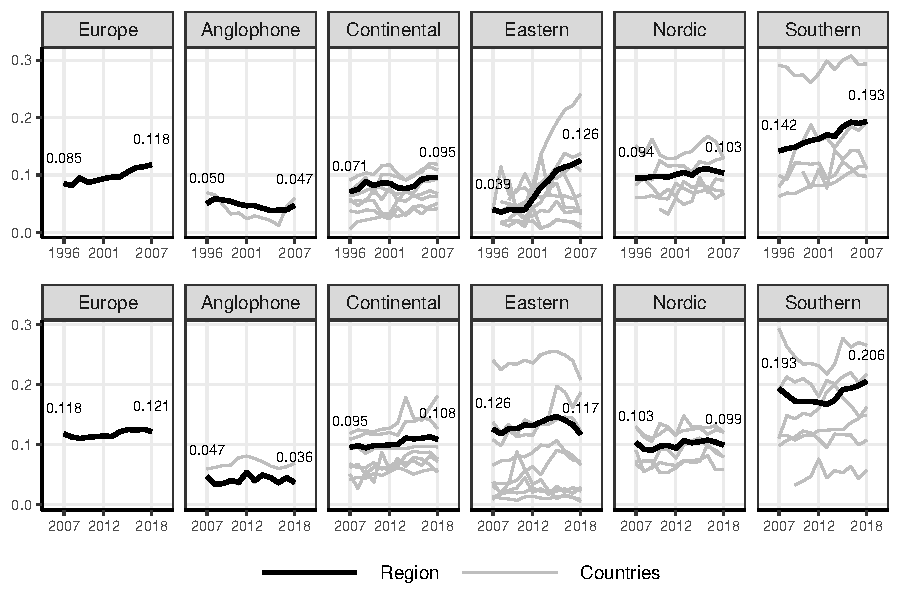
\includegraphics{../graphs/eu_lfs/graph_rate_region.pdf}}
    \label{graph_eu_lfs_rate_region}

    \footnotesize{Note: Authors calculations using LFS data.  Each cell shows the temporary employment rate for a given region, year, as shown by the thick, black line.  Country, region specifications are shown in table \ref{table_country_panel_years} in Appendix \ref{appendix_tables}.  Before 2007, levels are rising.  After 2007, levels are constant.  In the Eastern region, Poland stands out, with high and rising levels before 2007, but stagnating levels afterward.  In the Southern region, Spain stands out, with high, but declining levels, especially after 2007.  Italy and the Netherlands are among the few countries with high and rising levels before and after 2007.}
\end{figure}


\begin{sidewaysfigure}[htp!]
    \caption{Temporary employment rate over time, by demographic group (1996 - 2007)}
    \resizebox{\textwidth}{!}{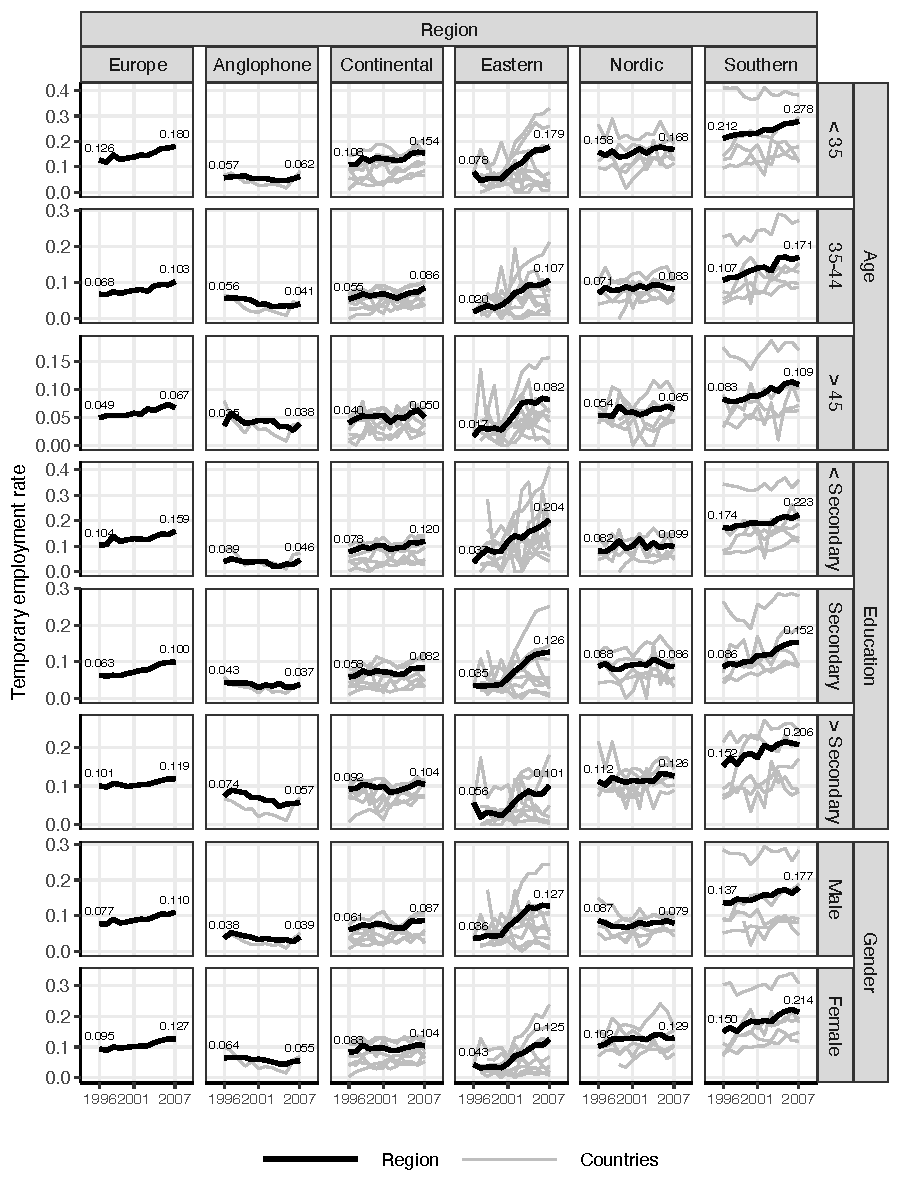
\includegraphics{../graphs/eu_lfs/graph_ftc_rate_region_country_group_period_1.pdf}}
    \label{graph_eu_lfs_pct_combo_1}
    \footnotesize{Note: Authors calculations using LFS data.  Each cell shows the temporary employment rate for a given region, year, demographic group.  For easier interpretation, highlighted subplots indicate where the temporary employment rate rose at least 1 percentage point and 10\% between 1996 and 2007.  Before 2007, the temporary employment rate is rising in almost every region and subgroup, except in the Anglophone and Nordic regions and among those with higher levels of education.}
\end{sidewaysfigure}

\begin{sidewaysfigure}[htp!]
    \caption{Temporary employment rate over time, by demographic group (2007 - 2019)}
    \resizebox{\textwidth}{!}{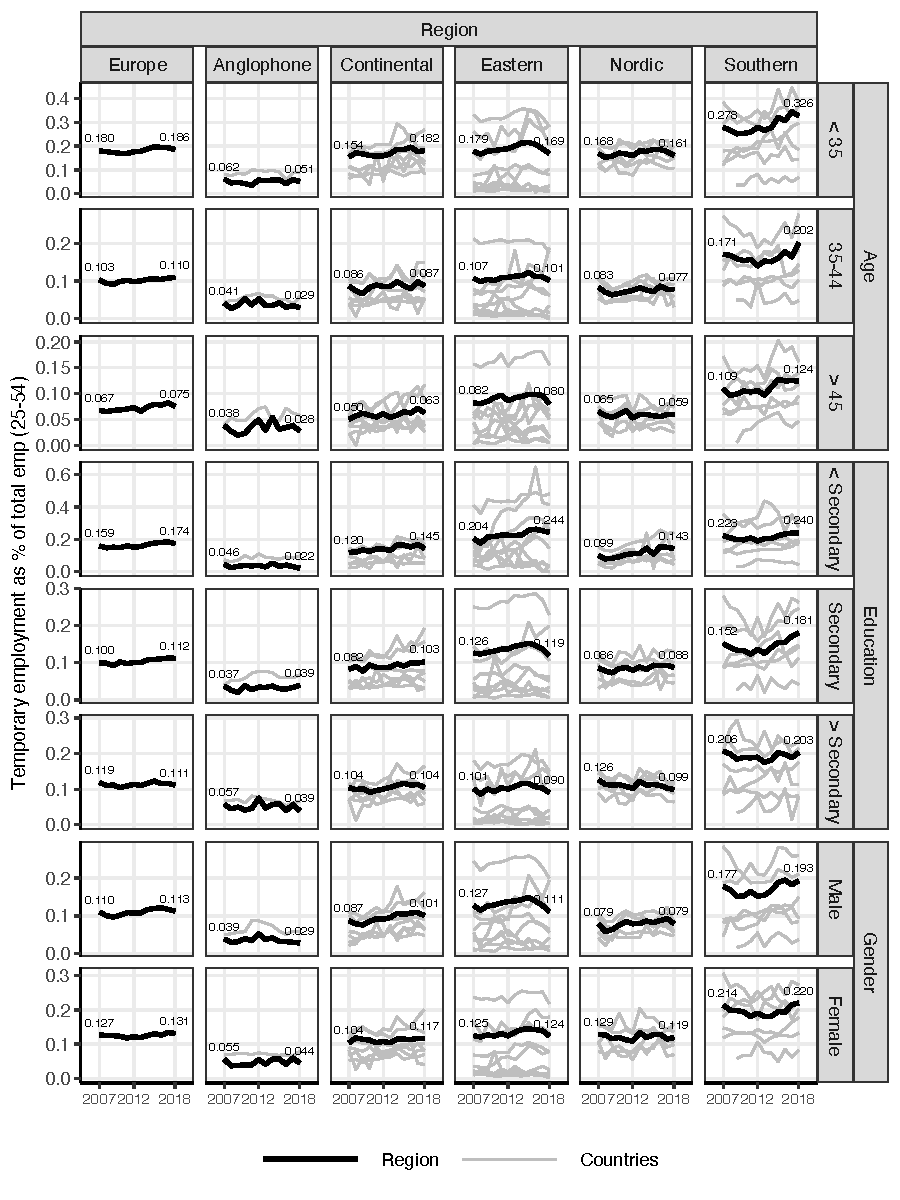
\includegraphics{../graphs/eu_lfs/graph_ftc_rate_region_country_group_period_2.pdf}}
    \label{graph_eu_lfs_pct_combo_2}    
    \footnotesize{Note: Authors calculations using LFS data.  Each cell shows the temporary employment rate for a given region, year, demographic group.  For easier interpretation, highlighted subplots indicate where the temporary employment rate rose at least 1 percentage points and 10\% between 2007 and 2019. After 2007, the temporary employment rate is constant within almost all demographic groups and regions.  However, there are two exceptions.  In the Southern region, the rate continues to rise in every demographic group, except those with higher levels of education.  Further, among those with lower levels of education, the rate continues to rise in every region, except the Anglophone region.}
\end{sidewaysfigure}

% Graphs - SILC

\clearpage
\begin{sidewaysfigure}[htp!]
    \caption{Predicted probability of a temporary contract}
    \resizebox{\textwidth}{!}{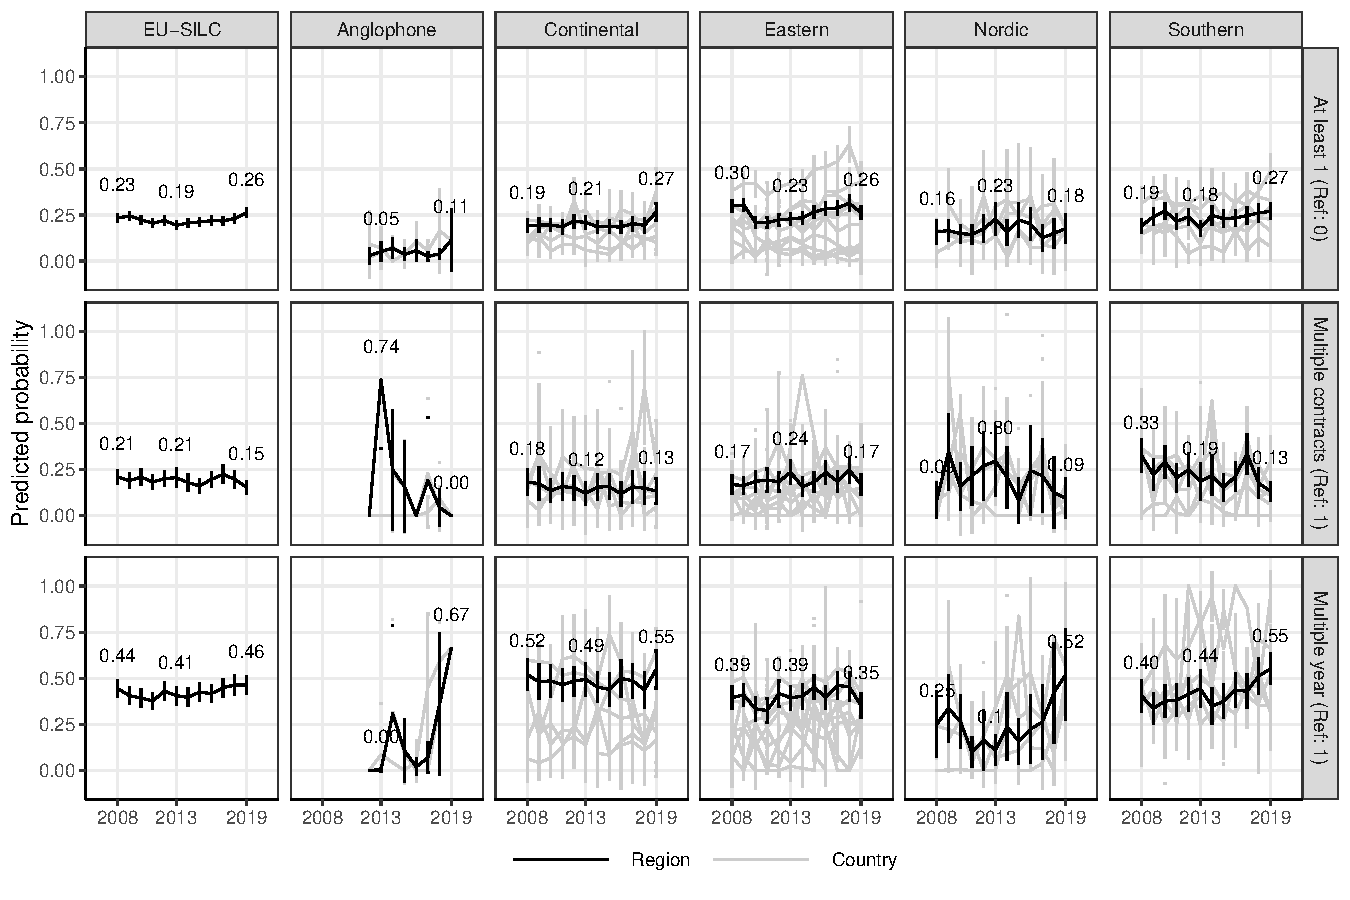
\includegraphics{../graphs/eu_silc/graph_eu_silc_glm_yhat_wt.pdf}}
    \label{graph_glm_yhat}
    \footnotesize{Note: Authors calculations using SILC data.  First row plots the probability of experiencing at least one temporary contract (ref: 0).  Second row plots the probability of experiencing multiple temporary contracts (ref: 1).  Third row plots the probability of experiencing a temporary contract that is multiple years long (ref: 1).  The interpretation is that temporary employment risk is rising, but the relative insecurity of temporary employment may be declining as the risk of receiving a multi-year contract is rising and the risk of receiving multiple contracts is constant or declining.}
\end{sidewaysfigure}

% Graphs - average marginal effect
\begin{sidewaysfigure}[htp!]
    \caption{AME of main effects on the probability of experiencing a temporary contract}
    \resizebox{\textwidth}{!}{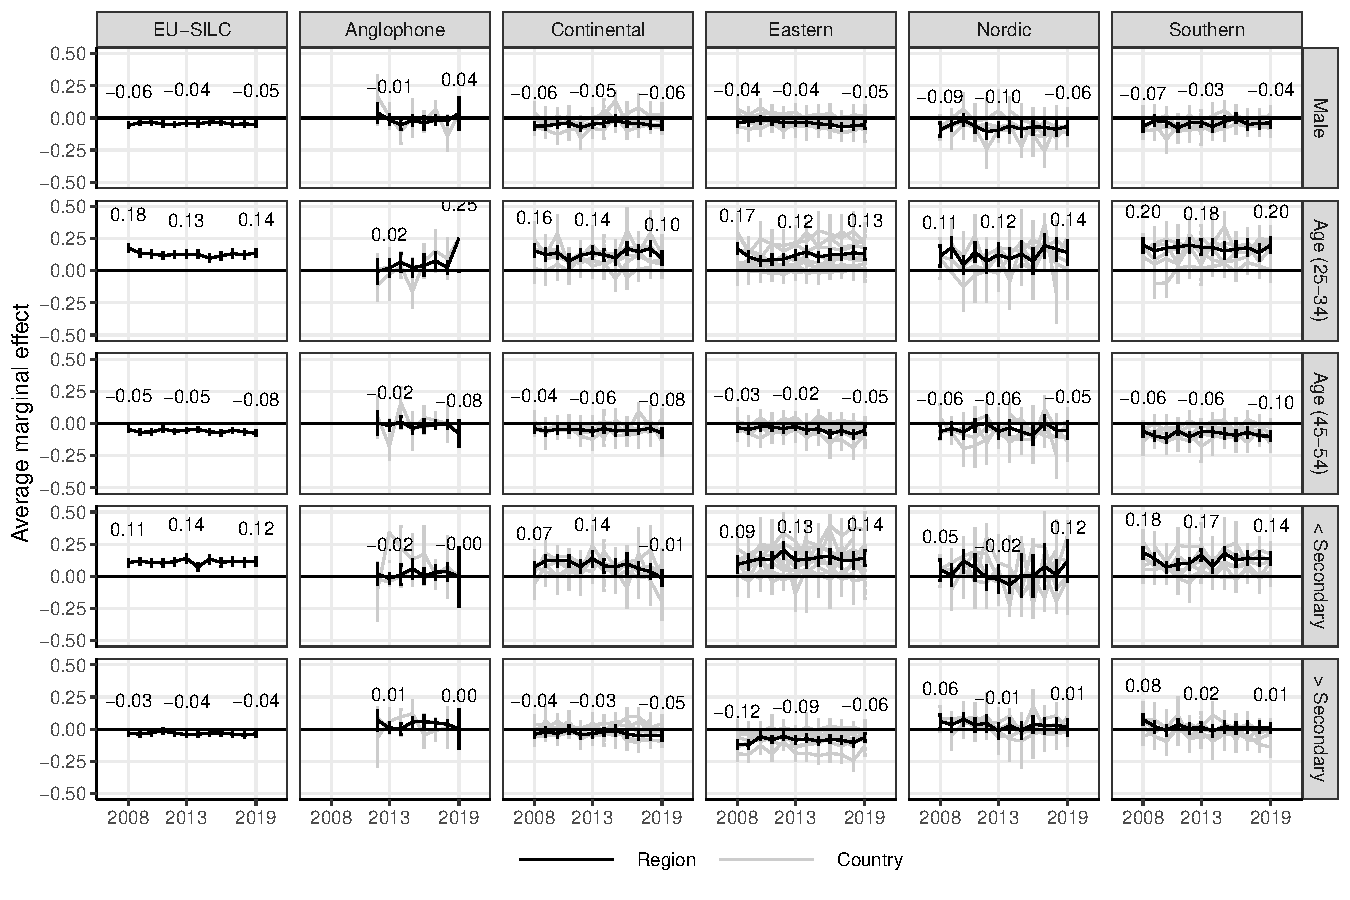
\includegraphics{../graphs/eu_silc/graph_eu_silc_glm_mfx_ever_wt.pdf}}
    \label{graph_glm_mfx_ever}
    \footnotesize{Note: Authors calculations using SILC data.  Plots the average marginal effect of independent variables on the probability of experiencing at least 1 temporary contract (ref: 0).  Between groups, risk is higher among women, younger workers, and those with lower levels of education.  However, within groups, there is little change in the demographic distribution of that rising risk.}
\end{sidewaysfigure}

\clearpage
\begin{sidewaysfigure}[htp!]
    \caption{AME of main effects on the number of temporary contracts}
    \resizebox{\textwidth}{!}{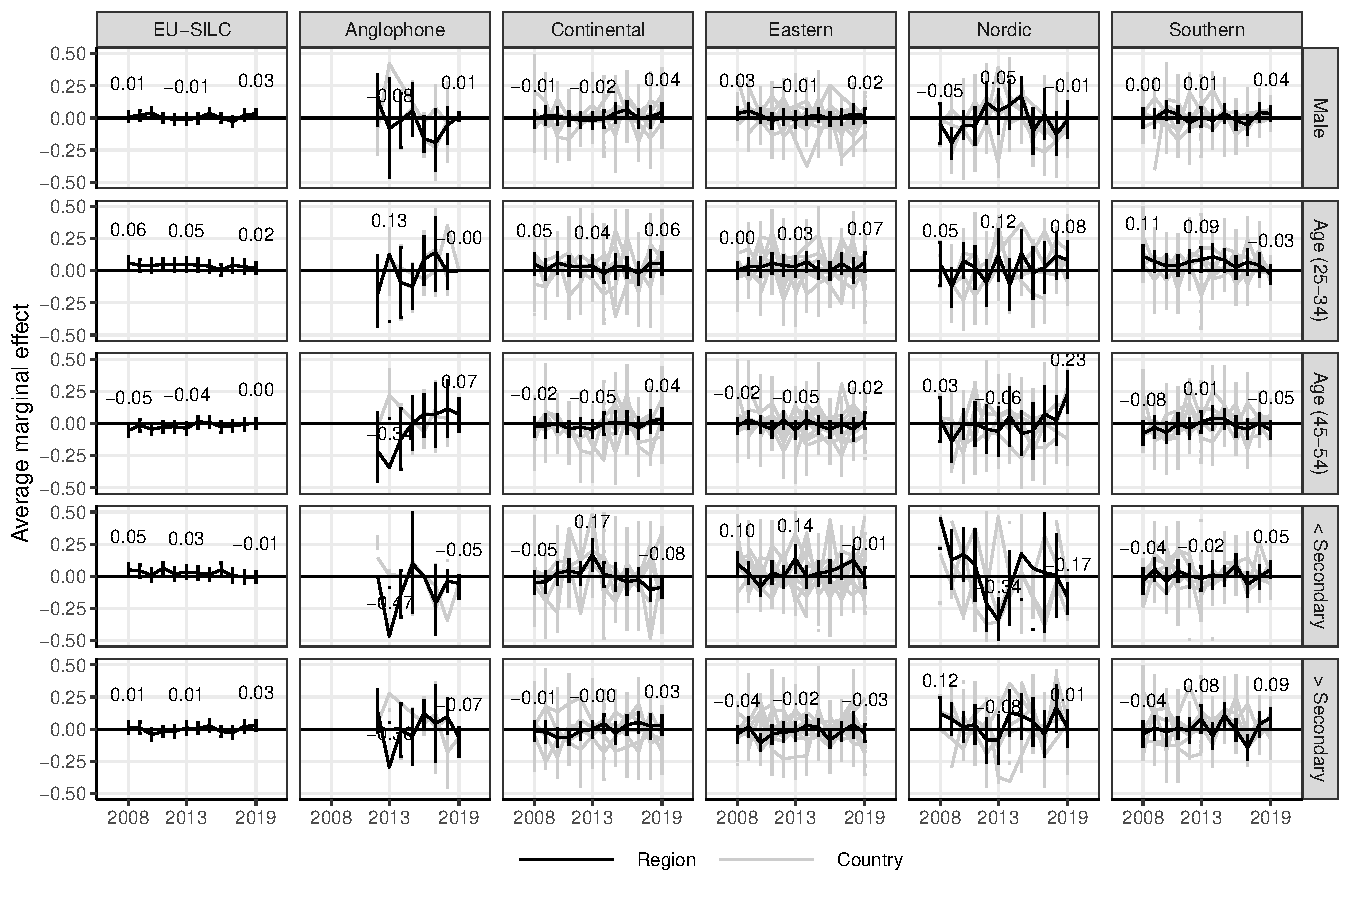
\includegraphics{../graphs/eu_silc/graph_eu_silc_glm_mfx_num_wt.pdf}}
    \label{graph_glm_mfx_num}
    \footnotesize{Note: Authors calculations using SILC data.  Plots the average marginal effect of independent variables on the probability of experiencing at least 2 temporary contracts (ref: 1).  In general, risk of multiple contracts is distributed equally between demographic groups.  Further, there is little change in the distribution of risk within demographic groups.}
\end{sidewaysfigure}

\clearpage
\begin{sidewaysfigure}[htp!]
    \caption{AME of main effects on the duration of temporary contracts}
    \resizebox{\textwidth}{!}{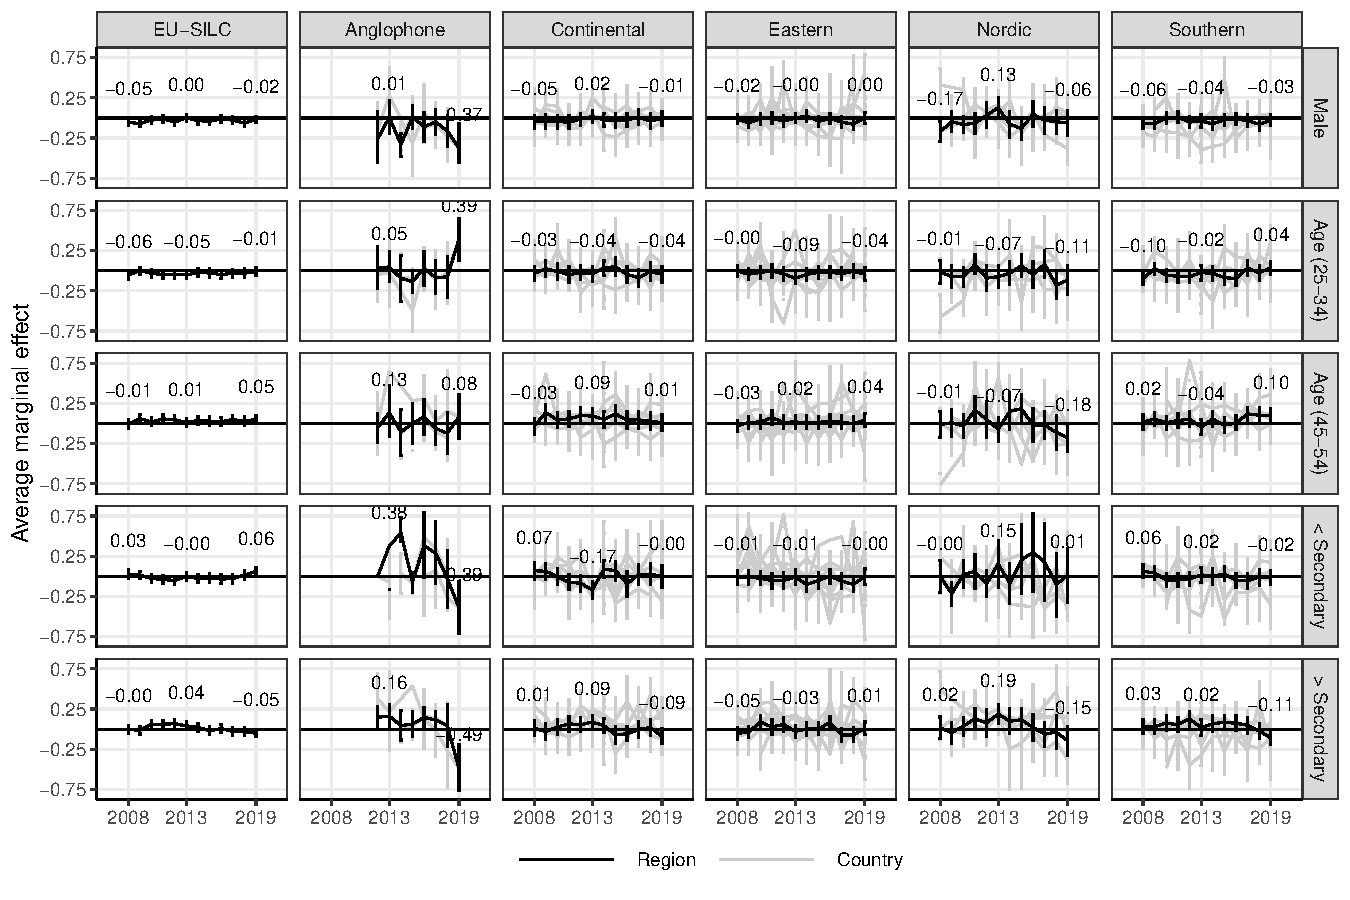
\includegraphics{../graphs/eu_silc/graph_eu_silc_glm_mfx_dur_wt.pdf}}
    \label{graph_glm_mfx_dur}
    \footnotesize{Note: Authors calculations using SILC data.  Plots the average marginal effect of independent variables on the probability of experiencing a temporary contract that is at least 2 years long (ref: 1). In general, risk of multi-year contracts is distributed equally between demographic groups.  Further, there is little change in the distribution of risk within demographic groups.}
\end{sidewaysfigure}


%%%%%%%%%%%%%%%%%%%%%%%%%%%%%%%%
% BIBLIOGRAPHY
%%%%%%%%%%%%%%%%%%%%%%%%%%%%%%%%

\clearpage
\singlespacing
\bibliographystyle{apalike2}
\bibliography{references}

%%%%%%%%%%%%%%%%%%%%%%%%%%
%APPENDIX
%%%%%%%%%%%%%%%%%%%%%%%%%%

\clearpage
\appendix
\setcounter{table}{0}
\setcounter{figure}{0}
\renewcommand*\thetable{\Alph{section}.\arabic{table}}
\renewcommand*\thefigure{\Alph{section}.\arabic{figure}}
\renewcommand{\theHfigure}{\Alph{section}.\arabic{table}}
\renewcommand{\theHtable}{\Alph{section}.\arabic{figure}}

\section{Appendix: Sample selection}
\label{appendix_sample}

We apply the following sample selection criteria to the EU-SILC, as shown in table \ref{tables_steps_silc_4}.  There are three main filters.  First, we apply country, panel-level filters.  We restrict all panels to study windows that are four-years long.  While the majority of countries use a four-year long panel, a few use longer study windows.  We exclude country, panel waves with a temporary employment rate of zero or missing.  This affects three countries, Denmark, the United Kingdom, and Iceland.\footnote{Denmark in years between 2005 and 2010 (panel waves 2008 to 2013), the United Kingdom in 2008 (panel waves 2008 to 2011), and Iceland in 2009 (2009 panel waves).}  Furthermore, we exclude countries with less than 3 panel waves because 3 periods are necessary to create a trend.  This only affects Germany, which is only present in panel waves 2018 and 2019.

We use 12 panel waves, between 2008 and 2019.  2019 is the most recent year data is available.  Waves prior to the 2007 panel wave only include three years of observational data and the 2007 panel wave only includes 15 countries, compared to 25 or more countries in the other surveys.  Further, after all sample selection criteria are applied, there are only four countries in the 2007 panel wave, compared to 18 in the 2008 panel wave.  The result is 13.502.253 observations in 346 country, panel waves.  

Second, we apply individual-level filters.  The data includes individuals who are prime age (25-54), for the same reasons about the relationship between (in)voluntariness and age with respect to the LFS data, active labor market participants, and have a non zero personal weight.\footnote{There are two exceptions.  In the Netherlands, in panel waves 2016 -- 2019, the personal weight for all observations in the first year of a given panel wave is zero.  Similarly, in Norway, beginning with the 2010 panel waves, only last observation in panel period has personal weight greater than 0.  In these country, panel waves, we recode the personal base weight for these observations in these years as 1 and keep the observations, conditional on meeting all other criteria.}  We exclude individuals who were never employed in a four-year panel wave, otherwise there is no possibility of experiencing temporary employment.  We drop observations with missing values on education, gender, age, and contract type.  The result is 3.675.604 observations in 346 country, panel waves in the sample. 

Third and finally, we apply individual, panel-level filters.  The data only include individuals who are observable in each year of a given four-year panel wave.  Further, we exclude observations with missing or zero longitudinal panel weights, which weights for the inverse probability of being in the sample for the entire panel wave.  This leaves 1.058.840 total observations (264.710 unique observations) in 325 country, panel waves.  This is our `main' dataset.  We note that while not every country is in every panel wave, of the 31 countries in the sample, 23 countries are in at least nine panel waves, as shown in table \ref{table_country_panel_years}.  

To examine our three outcomes of interest, we create three sub datasets from the main dataset.  The first dependent variable is experiencing at least one temporary contract in a given four-year panel wave (i.e. ever).  The reference is an individual who does not experience a temporary contract (i.e. never).  To estimate this outcome, we aggregate the main dataset so each individual is present once in a given country, panel wave.  The result is dataset \emph{A} with 264.710 person, country, panel observations.  

Next, we determine temporary employment `spells' in order to estimate the probability of experiencing temporary employment, by the number and duration of temporary contracts.  We calculate temporary employment spells for each individual in a given country, panel wave using a variable in the dataset that asks, ``Change of job since last year?''  If an individual had a temporary contract in two consecutive time periods, but did not change jobs, then they had one temporary contract for two years.  By contrast, if an individual in two consecutive time periods had a temporary contract, but did change jobs, then they had two temporary contracts, each of which was one year.

The second dependent variable is experiencing two or more, i.e. multiple, temporary contracts in a given panel wave.  The reference is experiencing one, single temporary contract in that same panel wave.  To examine this outcome, we filter from dataset \emph{A} on the condition of ever experiencing temporary employment.  The result is dataset \emph{B} with 48.940 person, country, panel wave observations.  

The third dependent variable is experiencing a temporary contract that is two or more years long, i.e. multiple years.  The reference group is experiencing a temporary contract that is one, single year long.  To examine this outcome, we aggregate the main dataset so each spell of temporary employment is present once in a given country, panel wave, but an individual with multiple spells is present as many times as they have spells in a given country, panel wave.  Further, we filter on the condition of ever experiencing temporary employment.  The result is dataset \emph{C} with 59.582 person-spell, country, panel observations. 

We exclude variables related to income, occupation, and industry.  While including these additional variables into our analysis would improve model fit, it is not clear the degree to which these variables are related to the individual, job, or structural conditions.  For example, in Germany, occupational closure in the form of tasks and credentials are important determinants of temporary employment levels within a given occupation, ranging from 0 to 64 percent \citep{stuth_2017}.  We also do not control for individual self-selection into temporary employment.  Further, instead of relying on a single, unified, multi-level models, we use separate regression models for each panel wave in each country.  In so doing, we ensure that results are a reflection of the data, not model specification.

We use the methods and data describe above to quantify inequalities in temporary employment trends over time as well as between and within countries and demographic groups.  The goal is not to causally isolate an ``effect'' of country and demographic groups on temporary employment risk net of a large number of control variables, nor the consequences of temporary employment, as other research does.  Instead, the primary goal is descriptive.  Results provide a more accurate and representative accounting of levels and trends in temporary employment rate and risk than is otherwise reported, which helps to isolate the source of rising insecurity associated with temporary employment.  Replication files are made available by the authors on GitHub.

\subsection{Sensitivity}

Here, we address several important issues of sensitivity, which we divide into two main parts.  One main part is the sensitivity of the results within a given data set to our particular sample selection criteria.  With respect to the LFS, conditional on being a prime-age worker (25-54) and employed, the other selection criteria reduce the sample by 23.5\% (as shown in table \ref{tables_steps_lfs}).  Of these criteria, the most important one is a contract type, which accounts 17 percentage points.  While contract type is an essential variable required to determine temporary employment rate, results are not sensitive to the inclusion or exclusion of the other selection criteria.  

With respect to the SILC, the most important criteria is the requirement that observations be in the sample for all 4 years of a panel period.  This reduces the sample by 71\% (as shown in table \ref{tables_steps_silc_4}).  Alternatively, if we only require an individual to be in the first 2 years of a 4 year panel period, we only lose 37\% of all cases (as shown in table \ref{tables_steps_silc_2}).  While results are qualitatively similar, as shown in figure \ref{graph_eu_silc_compare_2_4_year_panel}, we use a longer time period owing to the application of a life course approach.  Further, results are qualitatively similar using unadjusted, non-parametric data, as shown in figure \ref{graph_eu_silc_compare_2_4_year_panel}.  

The second main part is issue of whether the results are sensitive to the choice of data set used.  Or, put another way, what is the degree to which the samples from the two data sets are comparable?  One way the samples are different is that the LFS sample only include those who are employed, which is how one calculates the temporary employment rate, while the SILC sample include all labour force participants, employed or unemployed.  We compare the temporary employment rate among the employed population to the rate among the employed and unemployed.  Trends are qualitatively similar, as shown in \ref{graph_rate_region_compare_lmp}.  

Another issue of comparison is that it is possible to use the SILC data in a cross-sectional form, as we described above, as well as the 4-year sample we use for our analysis, and the 2-year sample we use for sensitivity.  We compare the annual temporary employment rate between all three versions of SILC sample to LFS sample.  Results are qualitatively similar, as shown in figure \ref{graph_eu_silc_compare_SILC_LFS}.  


\clearpage
\section{Appendix: Tables}
\label{appendix_tables}

\begin{table}[h!]	
	\caption{Sample selection (EU-SILC, 4 year panel)}
    \resizebox{\textwidth}{!}{\begin{tabular}{l>{\raggedright\arraybackslash}p{1in}ll>{\raggedright\arraybackslash}p{4in}}
   \\[-1.8ex]\hline \\ 
 [-1.8ex]
\multicolumn{1}{l}{Step} & 
\multicolumn{1}{>{\raggedright\arraybackslash}p{1in}}{Country, panel periods} &
\multicolumn{1}{>{\raggedright\arraybackslash}p{1in}}{Unique observations} &
\multicolumn{1}{l}{\% $\Delta$} & 
\multicolumn{1}{l}{Notes} 
\\  

 \hline
0 & 377 & 5.961.876 &  & Raw data \\ 
  1 & 346 & 5.492.337 & -8\% & Country panel filters: Drop 2007 panel period.  Every panel period can only have four years.  Each country, panel, year must have non-missing temporary employment rate $>$ 0 \\ 
  2 & 346 & 2.278.772 & -59\% & Individual filters: prime age (25 - 54), active labor market participation (employed or unemployed), personal weight $>$ 0 \\ 
  3 & 346 & 2.082.421 & -9\% & Must be employed at least once \\ 
  4 & 346 & 1.588.269 & -24\% & Case-wise deletion of missing variables on education, gender, age, and contract type \\ 
  5 & 331 & 267.846 & -83\% & Individuals in each year of 4 year panel period \\ 
  6 & 325 & 264.710 & -1\% & Must have 4 year longitudinal weight (`Main dataset') \\ 
   \hline 
7 & Dataset \emph{A} & 264.710 &  & Main data:  One observation per individual, panel wave (ever) \\ 
  8 & Dataset \emph{B} & 48.940 &  & Dataset \emph{A}:$|>= 1$ temporary contract (number) \\ 
  9 & Dataset \emph{C} & 59.582 &  & Main data:$|>= 1$ temporary contract, one observation per spell, panel wave (duration) \\ 
   \hline 
 \hline 
\end{tabular}
}
    \label{tables_steps_silc_4}
\end{table}

\begin{sidewaystable}[h!]
    \caption{Number of observations per country, panel wave (EU-SILC, 4 year panel)}
    \footnotesize
    \resizebox{\textwidth}{!}{\begin{tabular}{lrrrrrrrrrrrrrr}
   \\[-1.8ex]\hline \\ 
 [-1.8ex] \multicolumn{1}{l}{Country} & \multicolumn{12}{l}{Four-year panel period ending} & \multicolumn{2}{l}{Total} \\ 

                    \cmidrule(r){1-1} \cmidrule(r){2-13} \cmidrule(r){14-15} 

            & 2008 & 2009 & 2010 & 2011 & 2012 & 2013 & 2014 & 2015 & 2016 & 2017 & 2018 & 2019 & Observations & Periods \\ 
 \hline
\\[-1.8ex]
  Anglophone countries: &  &  &  &  & 1.164 & 2.832 & 3.076 & 3.900 & 3.504 & 5.820 & 5.632 & 840 & 26.768 &   8 \\ 
  \hspace{5mm} Ireland &  &  &  &  & 600 & 640 & 648 & 528 & 1.188 & 2.104 & 1.100 & 840 & 7.648 &   8 \\ 
  \hspace{5mm} United Kingdom &  &  &  &  & 564 & 2.192 & 2.428 & 3.372 & 2.316 & 3.716 & 4.532 &  & 19.120 &   7 \\ 
  \multicolumn{14}{l}{\phantom{empty}} \\
  Continental countries: & 19.900 & 25.220 & 27.640 & 27.396 & 29.232 & 22.392 & 24.076 & 23.420 & 23.572 & 22.220 & 20.344 & 20.628 & 286.040 &  12 \\ 
  \hspace{5mm} Austria & 2.424 & 2.388 & 2.552 & 2.504 & 3.040 & 2.832 & 2.460 & 2.432 & 2.356 & 2.540 & 2.328 & 2.664 & 30.520 &  12 \\ 
  \hspace{5mm} Belgium & 2.856 & 2.676 & 2.868 & 2.284 & 2.336 & 2.516 & 2.264 & 2.252 & 2.732 & 2.296 & 2.388 & 3.856 & 31.324 &  12 \\ 
  \hspace{5mm} France & 11.260 & 11.376 & 12.160 & 12.776 & 13.520 & 12.432 & 12.020 & 11.828 & 11.664 & 10.504 & 9.732 & 9.224 & 138.496 &  12 \\ 
  \hspace{5mm} Luxembourg &  & 6.808 & 6.980 & 7.052 & 7.748 & 1.860 & 1.932 & 1.880 & 2.028 & 1.792 & 1.220 & 2.284 & 41.584 &  11 \\ 
  \hspace{5mm} Netherlands & 3.360 & 1.972 & 3.080 & 2.780 & 2.588 & 2.752 & 2.744 & 2.376 & 2.416 & 2.276 & 2.012 & 2.600 & 30.956 &  12 \\ 
  \hspace{5mm} Switzerland &  &  &  &  &  &  & 2.656 & 2.652 & 2.376 & 2.812 & 2.664 &  & 13.160 &   5 \\ 
  \multicolumn{14}{l}{\phantom{empty}} \\
  Eastern countries: & 27.604 & 32.044 & 34.020 & 32.632 & 34.352 & 36.128 & 36.900 & 33.148 & 38.328 & 35.040 & 38.200 & 37.260 & 415.656 &  12 \\ 
  \hspace{5mm} Bulgaria &  & 1.664 & 1.684 & 2.892 & 3.240 & 2.576 & 2.456 & 2.388 & 6.384 & 6.208 & 5.980 & 6.200 & 41.672 &  11 \\ 
  \hspace{5mm} Croatia &  &  &  &  &  & 2.048 & 1.908 & 1.824 & 1.728 & 2.284 & 3.704 & 3.504 & 17.000 &   7 \\ 
  \hspace{5mm} Czechia & 7.692 & 6.756 & 5.076 & 3.392 & 4.700 & 4.696 & 4.424 & 3.508 & 3.628 & 3.748 & 3.928 & 3.964 & 55.512 &  12 \\ 
  \hspace{5mm} Estonia & 1.004 & 2.940 & 2.808 & 2.596 & 2.176 & 2.532 & 2.316 & 2.796 & 2.672 & 2.652 & 2.264 & 2.856 & 29.612 &  12 \\ 
  \hspace{5mm} Hungary & 3.336 & 3.532 & 3.756 & 3.196 & 4.240 & 3.528 & 6.332 & 2.820 & 3.060 & 3.160 & 2.708 & 2.252 & 41.920 &  12 \\ 
  \hspace{5mm} Latvia & 1.684 & 1.828 & 2.044 & 2.564 & 2.436 & 2.556 & 2.424 & 2.168 & 2.024 & 1.832 & 2.052 & 1.912 & 25.524 &  12 \\ 
  \hspace{5mm} Lithuania & 1.884 & 2.712 & 2.744 & 2.520 & 2.472 & 2.892 & 2.132 & 2.340 & 1.760 & 2.424 & 1.596 & 1.900 & 27.376 &  12 \\ 
  \hspace{5mm} Poland & 6.556 & 6.812 & 6.196 & 5.408 & 5.488 & 5.924 & 5.696 & 5.972 & 5.148 & 4.988 & 3.980 & 3.956 & 66.124 &  12 \\ 
  \hspace{5mm} Romania &  &  & 3.516 & 3.512 & 3.300 & 3.484 & 3.108 & 3.276 & 3.376 & 3.320 & 3.708 & 3.428 & 34.028 &  10 \\ 
  \hspace{5mm} Serbia &  &  &  &  &  &  &  &  & 2.648 & 2.456 & 2.660 & 2.604 & 10.368 &   4 \\ 
  \hspace{5mm} Slovakia & 3.440 & 3.660 & 4.064 & 4.024 & 3.988 & 3.684 & 3.888 & 3.728 & 3.892 &  & 3.652 &  & 38.020 &  10 \\ 
  \hspace{5mm} Slovenia & 2.008 & 2.140 & 2.132 & 2.528 & 2.312 & 2.208 & 2.216 & 2.328 & 2.008 & 1.968 & 1.968 & 4.684 & 28.500 &  12 \\ 
  \multicolumn{14}{l}{\phantom{empty}} \\
  Nordic countries: & 4.560 & 6.872 & 7.576 & 6.604 & 6.108 & 6.180 & 6.588 & 5.868 & 6.148 & 5.660 & 5.612 & 5.148 & 72.924 &  12 \\ 
  \hspace{5mm} Denmark &  &  &  &  &  &  & 808 & 1.192 & 1.148 & 976 & 764 & 880 & 5.768 &   6 \\ 
  \hspace{5mm} Finland &  & 1.372 & 1.388 & 1.320 & 1.064 & 2.020 & 2.104 & 1.944 & 2.040 & 1.924 & 1.948 & 1.864 & 18.988 &  11 \\ 
  \hspace{5mm} Iceland & 608 &  & 568 & 672 & 636 & 556 & 552 & 532 & 532 & 480 & 440 &  & 5.576 &  10 \\ 
  \hspace{5mm} Norway & 3.952 & 3.728 & 3.484 & 3.140 & 2.896 & 2.192 & 2.004 & 1.304 & 1.340 & 1.220 & 1.252 & 1.344 & 27.856 &  12 \\ 
  \hspace{5mm} Sweden &  & 1.772 & 2.136 & 1.472 & 1.512 & 1.412 & 1.120 & 896 & 1.088 & 1.060 & 1.208 & 1.060 & 14.736 &  11 \\ 
  \multicolumn{14}{l}{\phantom{empty}} \\
  Southern countries: & 16.904 & 20.744 & 21.588 & 20.104 & 18.988 & 19.444 & 18.960 & 20.780 & 21.396 & 21.796 & 28.204 & 28.544 & 257.452 &  12 \\ 
  \hspace{5mm} Cyprus & 2.160 & 2.124 & 1.928 & 1.712 & 1.768 & 3.520 & 2.376 & 3.384 & 1.996 & 2.532 & 2.348 & 2.472 & 28.320 &  12 \\ 
  \hspace{5mm} Greece &  & 2.248 & 1.764 & 2.188 & 1.764 & 1.376 & 1.072 & 1.264 & 2.596 & 2.832 & 6.980 & 5.264 & 29.348 &  11 \\ 
  \hspace{5mm} Italy & 7.316 & 6.996 & 7.700 & 6.736 & 5.648 & 4.904 & 6.144 & 6.136 & 6.132 & 6.012 & 4.468 & 7.744 & 75.936 &  12 \\ 
  \hspace{5mm} Malta &  & 1.292 & 1.200 & 1.096 & 1.100 & 1.632 & 1.964 & 1.696 & 2.080 & 1.804 & 1.828 & 1.692 & 17.384 &  11 \\ 
  \hspace{5mm} Portugal & 1.868 & 1.964 & 2.252 & 1.860 & 2.624 & 2.624 & 2.940 & 3.248 & 3.576 & 3.520 & 7.280 & 6.792 & 40.548 &  12 \\ 
  \hspace{5mm} Spain & 5.560 & 6.120 & 6.744 & 6.512 & 6.084 & 5.388 & 4.464 & 5.052 & 5.016 & 5.096 & 5.300 & 4.580 & 65.916 &  12 \\ 
  \multicolumn{14}{l}{\phantom{empty}} \\
  EU-SILC & 68.968 & 84.880 & 90.824 & 86.736 & 89.844 & 86.976 & 89.600 & 87.116 & 92.948 & 90.536 & 97.992 & 92.420 & 1.058.840 & 325 \\ 
   \hline\hline \\[-1.8ex] 
\end{tabular}
}
    \label{table_country_panel_years}
\end{sidewaystable}

\begin{table}[h!]   
    \caption{Sample selection (EU-LFS)}
    \resizebox{\textwidth}{!}{\begin{tabular}{l>{\raggedright\arraybackslash}p{1in}ll>{\raggedright\arraybackslash}p{4in}}
   \\[-1.8ex]\hline \\ 
 [-1.8ex]
\multicolumn{1}{l}{Step} & 
\multicolumn{1}{>{\raggedright\arraybackslash}p{1in}}{Country, year periods} &
\multicolumn{1}{l}{Observations} & 
\multicolumn{1}{l}{\% $\Delta$} & 
\multicolumn{1}{l}{Notes} 
\\  

 \hline
0 & 708 & 85.678.076 &  & Raw data \\ 
  1 & 708 & 27.105.901 & -68\% & Year $>=$ 1996, employed, prime age (25 - 54) \\ 
  2 & 706 & 22.582.555 & -17\% & Observable contract type \\ 
  3 & 698 & 22.247.241 & -1\% & Observable education \\ 
  4 & 698 & 20.768.195 & -7\% & Personal weight $>$ 0 \\ 
   \hline 
\end{tabular}
}
    \label{tables_steps_lfs}
\end{table}

\begin{table}[h!]	
	\caption{Sample selection (EU-SILC, 2 year panel), as comparable to table \ref{tables_steps_silc_4}}
    \resizebox{\textwidth}{!}{\begin{tabular}{l>{\raggedright\arraybackslash}p{1in}ll>{\raggedright\arraybackslash}p{4in}}
   \\[-1.8ex]\hline \\ 
 [-1.8ex]
\multicolumn{1}{l}{Step} & 
\multicolumn{1}{>{\raggedright\arraybackslash}p{1in}}{Country-panel periods} &
\multicolumn{1}{l}{Observations} & 
\multicolumn{1}{l}{\% $\Delta$} & 
\multicolumn{1}{l}{Notes} 
\\  

 \hline
0 & 377 & 14.724.687 &  & Raw data \\ 
  1 & 346 & 13.502.253 & -8\% & Country panel filters: Drop 2007 panel period.  Every panel period can only have four years.  Each country, panel, year must have non-missing temporary employment rate $>$ 0 \\ 
  2 & 346 & 5.234.565 & -61\% & Individual filters: prime age (25 - 54), active labor market participation (employed or unemployed), personal weight $>$ 0 \\ 
  3 & 346 & 4.887.435 & -7\% & Must be employed at least once \\ 
  4 & 346 & 3.675.604 & -25\% & Case-wise deletion of missing variables on education, gender, age, and contract type \\ 
  5 & 345 & 2.307.656 & -37\% & Individuals in first 2 years of 4 year panel period \\ 
  6 & 343 & 1.914.466 & -17\% & Must have 2 year longitudinal weight (`Main dataset') \\ 
   \hline 
7 & Dataset \emph{A} & 957.233 &  & Main data:  One observation per individual, panel wave (ever) \\ 
  8 & Dataset \emph{B} & 151.015 &  & Dataset \emph{A}:$|>= 1$ temporary contract (number) \\ 
  9 & Dataset \emph{C} & 162.716 &  & Main data:$|>= 1$ temporary contract, one observation per spell, panel wave (duration) \\ 
   \hline 
 \hline 
\end{tabular}
}
    \label{tables_steps_silc_2}
\end{table}

\clearpage
\section{Appendix: Figures}
\label{appendix_figures}

\begin{sidewaysfigure}[htp!]
    \caption{Replicate figure \ref{graph_glm_yhat} with different EU-SILC samples}
    \resizebox{\textwidth}{!}{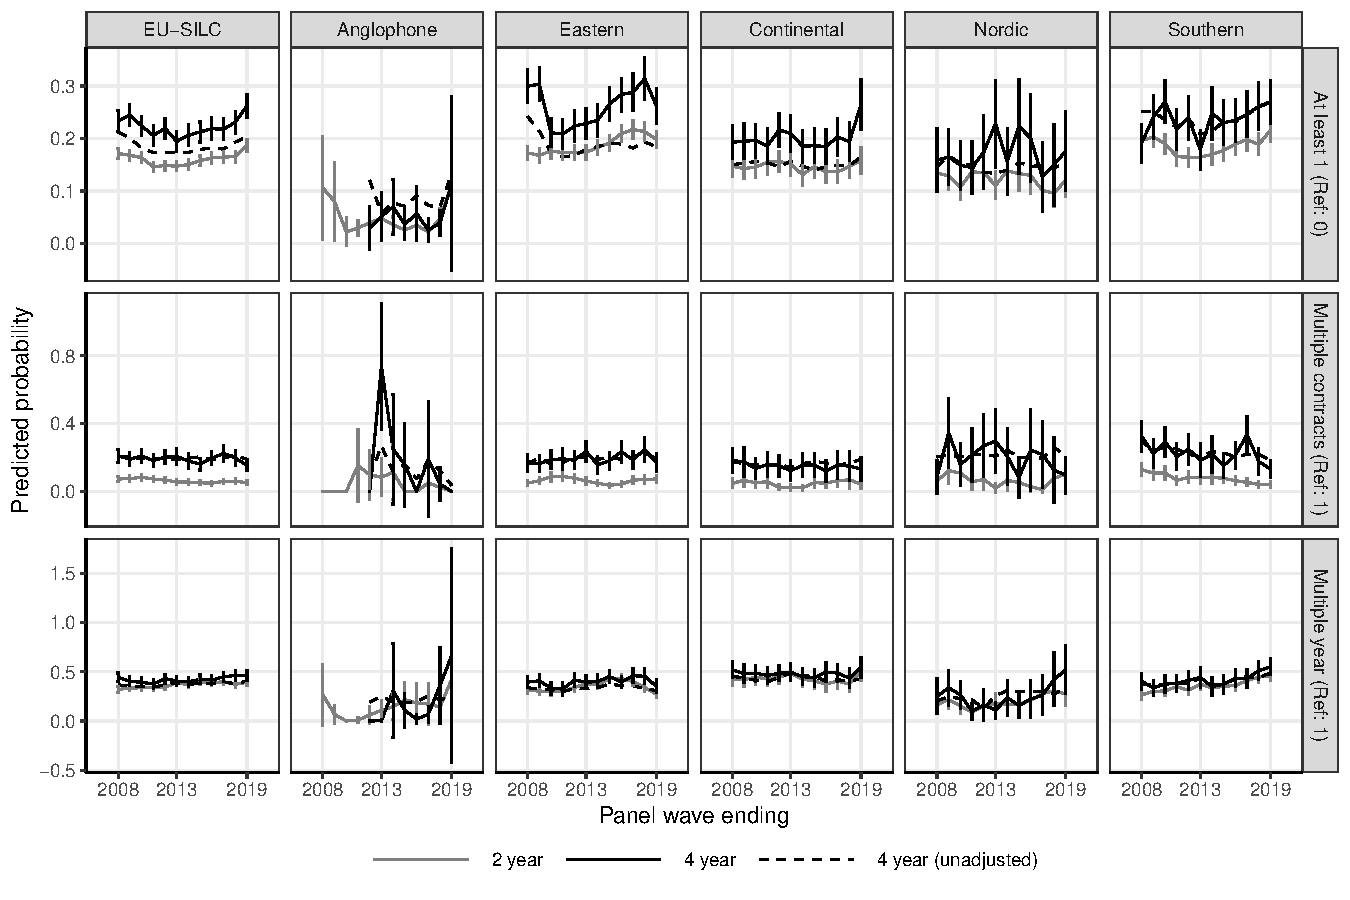
\includegraphics{../graphs/eu_silc/sensitivity/graph_eu_silc_compare_2_4_year_panel.pdf}}
    \label{graph_eu_silc_compare_2_4_year_panel}
    \footnotesize{Note: Authors calculations using SILC data.  The black, solid line is used in the main paper.  The gray, solid line applies the same sample selection strategy and applies the same model, but using a 2-year sample.  The black, dotted line uses the same sample selection strategy as the paper, but is not model adjusted.  Results are qualitatively similar.  The interpretation is that results are not a reflection of bias from model specification or sample attrition.}
\end{sidewaysfigure}

\begin{figure}[htp!]
    \caption{Replicate figure \ref{graph_eu_lfs_rate_region}, with different definitions of temporary employment rate}
    \resizebox{\textwidth}{!}{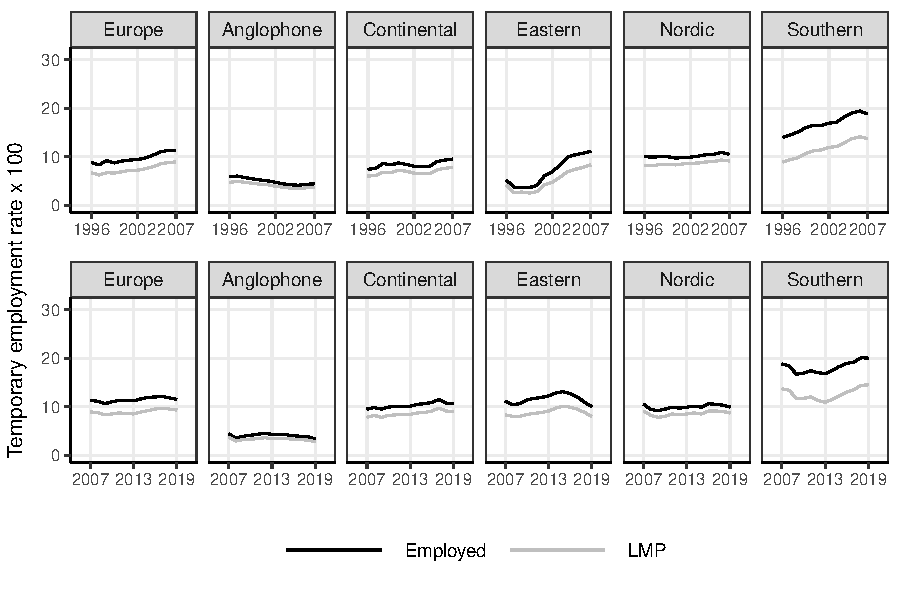
\includegraphics{../graphs/eu_lfs/sensitivity/graph_rate_region_compare_lmp.pdf}}
    \label{graph_rate_region_compare_lmp}
    \footnotesize{Note: Authors calculations using LFS data.  Each cell shows the temporary employment rate for a given region, year.  Black line shows the temporary employment rate among those who are employed in the LFS.  This is the standard way to calculate the temporary employment rate.  Gray line shows the temporary employment rate among those who are employed or unemployed in the LFS, i.e. labour market participants (LMP).  This is similar to the SILC sample.  The two lines are similar, although the rate is always lower using the sample of LMP, as we would expect.  The interpretation is that the temporary employment rate in the LFS is not driven by the sample selection strategy.}
\end{figure}

\begin{sidewaysfigure}[htp!]
    \caption{Comparing temporary employment rate across different data sources}
    \resizebox{\textwidth}{!}{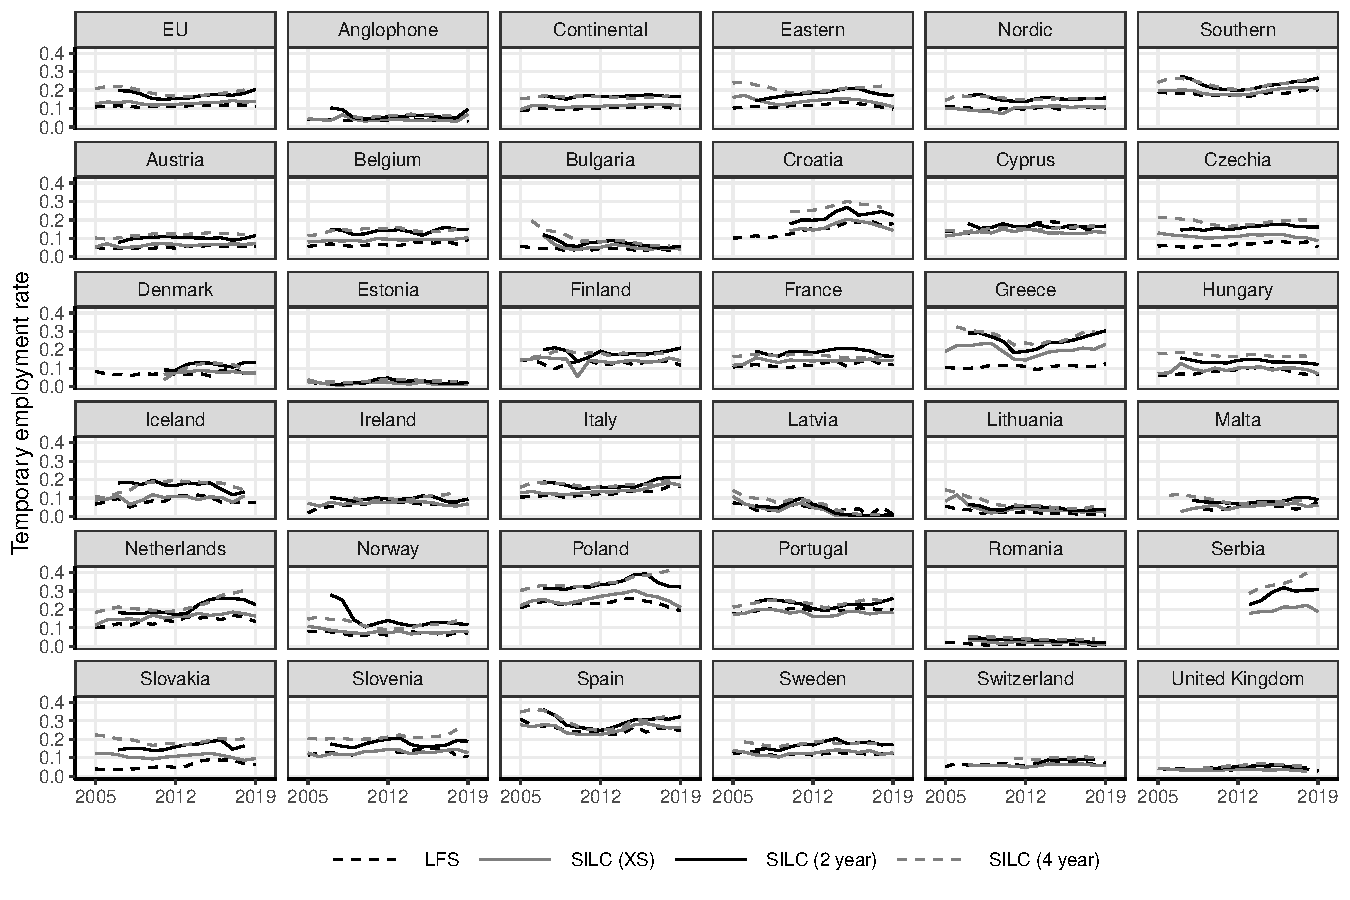
\includegraphics{../graphs/eu_silc/sensitivity/graph_eu_silc_compare_SILC_LFS.pdf}}
    \label{graph_eu_silc_compare_SILC_LFS}
    \footnotesize{Note: Authors calculations using LFS/SILC data.  Black, dotted line is temporary employment rate from cross-sectional, LFS data.  Gray, solid line is temporary employment rate from cross-sectional, SILC data.  Black, solid line is temporary employment rate from 2-year SILC sample.  Black, dashed line is temporary employment rate from 4-year SILC sample.  Temporary employment rate is similar, regardless of data type}
\end{sidewaysfigure}

\begin{figure}[htp!]
    \caption{Predicted probability of at least 1 temporary contract, by country}
    \resizebox{\textwidth}{!}{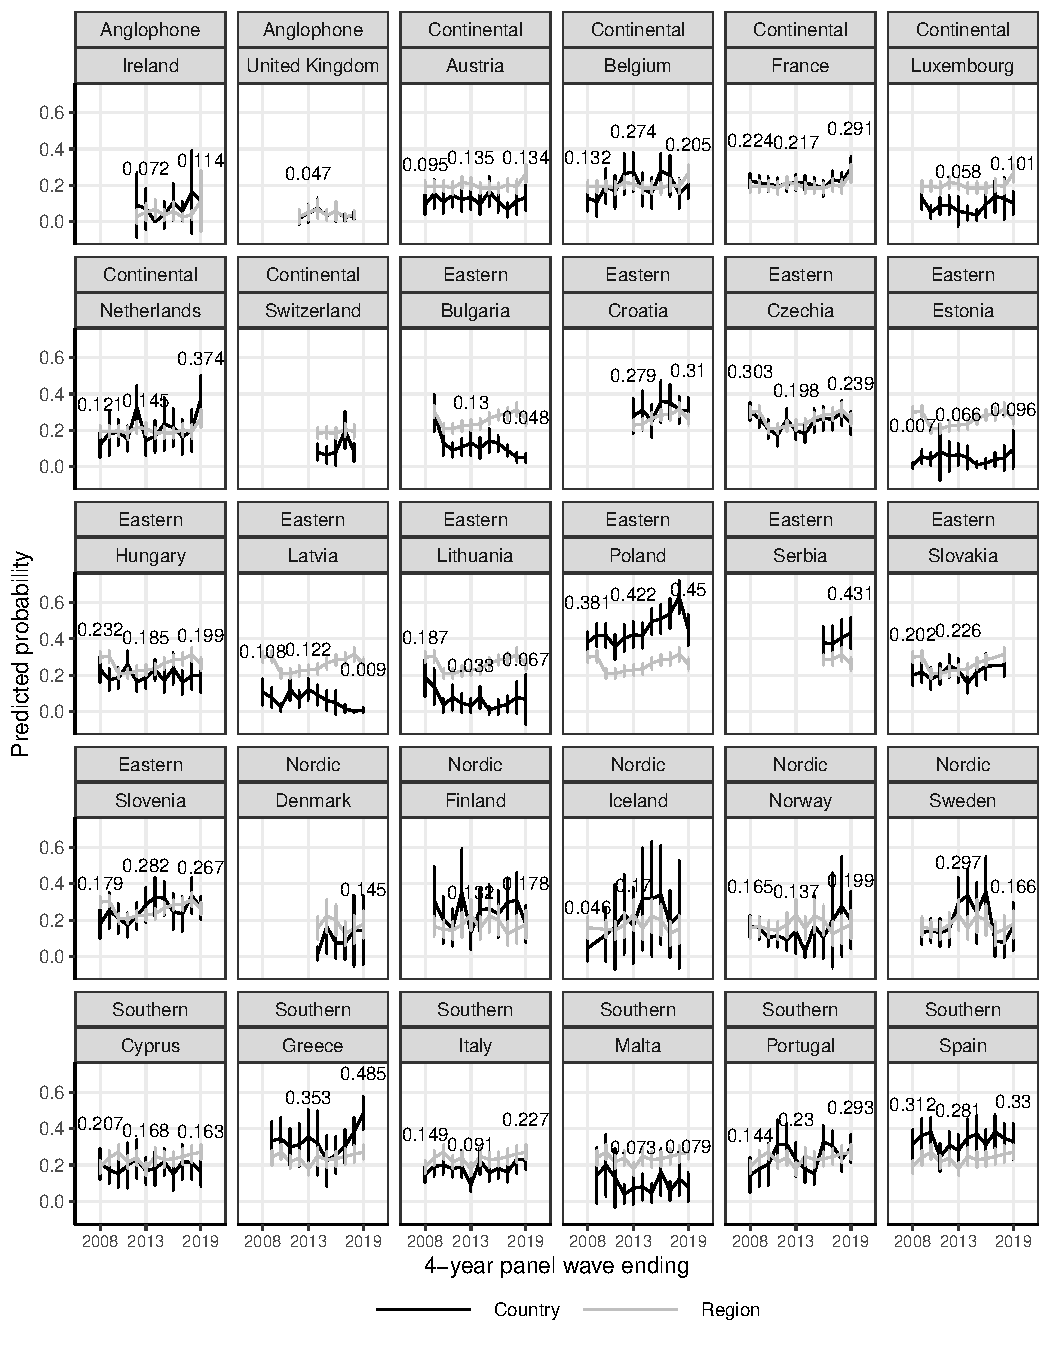
\includegraphics{../graphs/eu_silc/graph_eu_silc_glm_yhat_ever_country.pdf}}
    \label{graph_eu_silc_glm_yhat_ever_country}
    \footnotesize{Note: Authors calculations using SILC data.  Plots the probability of experiencing at least one temporary contract (ref: 0) from row 1 in figure \ref{graph_glm_yhat}, but with more country-level detail.  Each subplot is its own country.  Gray line is region-level.  Black line is country-level.}
\end{figure}

\begin{figure}[htp!]
    \caption{Predicted probability of a temporary contract (number), by country}
    \resizebox{\textwidth}{!}{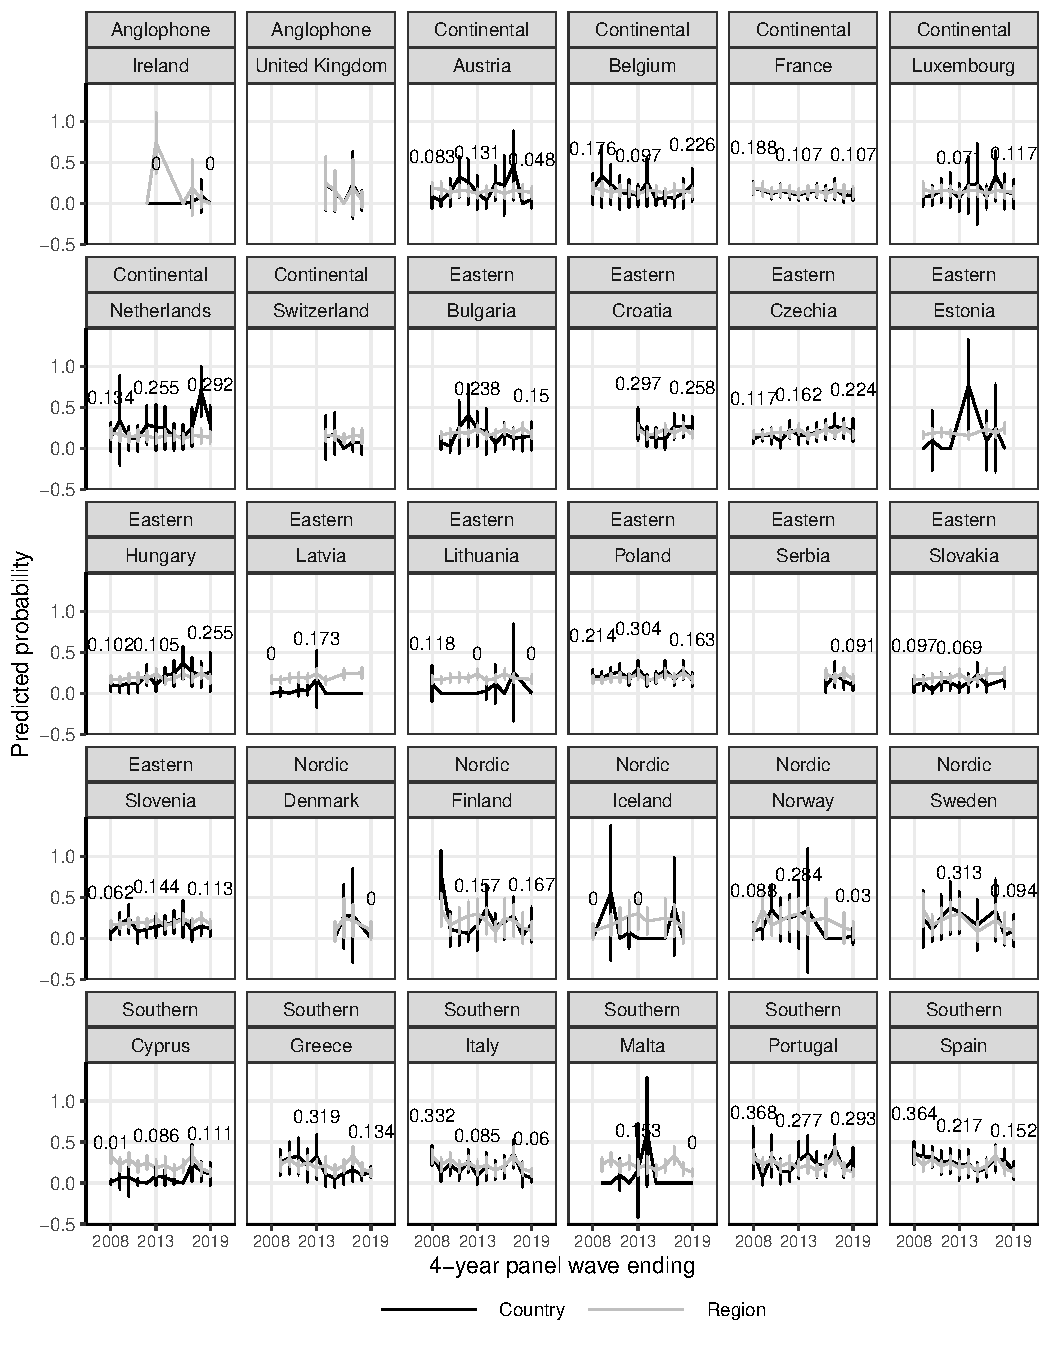
\includegraphics{../graphs/eu_silc/graph_eu_silc_glm_yhat_num_country.pdf}}
    \label{graph_eu_silc_glm_yhat_num_country}
    \footnotesize{Note: Authors calculations using SILC data.  Plots the probability of experiencing multiple temporary contracts (ref: 1) from row 2 in figure \ref{graph_glm_yhat}, but with more country-level detail.  Each subplot is its own country.  Gray line is region-level.  Black line is country-level.}
\end{figure}

\begin{figure}[htp!]
    \caption{Predicted probability of a temporary contract (duration), by country}
    \resizebox{\textwidth}{!}{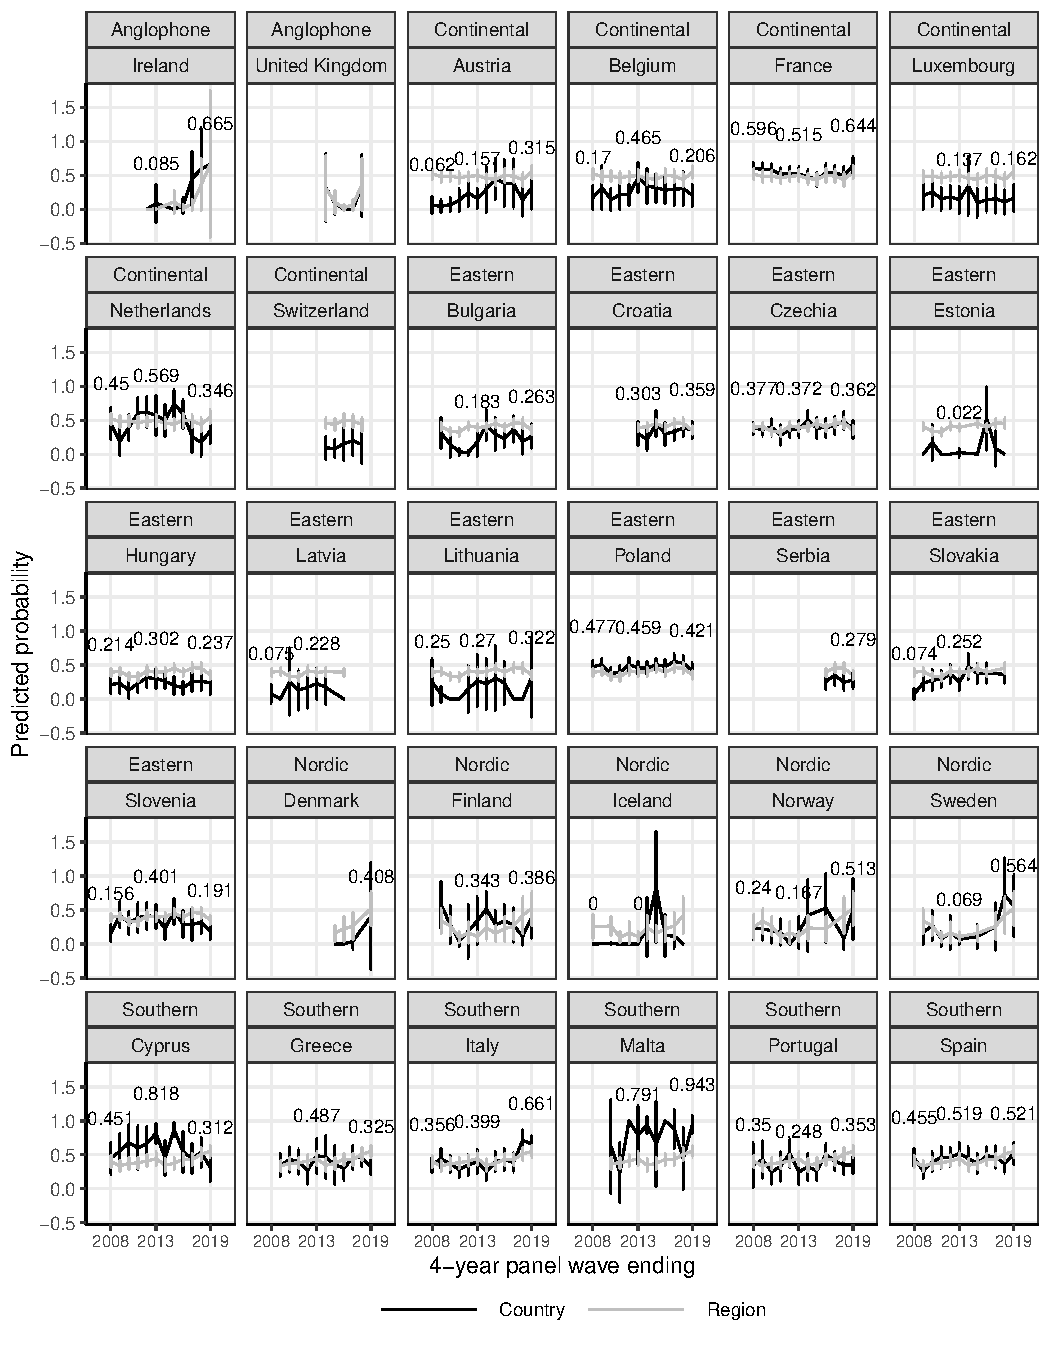
\includegraphics{../graphs/eu_silc/graph_eu_silc_glm_yhat_dur_country.pdf}}
    \label{graph_eu_silc_glm_yhat_dur_country}
    \footnotesize{Note: Authors calculations using SILC data.  Plots the probability of experiencing a temporary contract that is multiple years long (ref: 1) from row 3 in figure \ref{graph_glm_yhat}, but with more country-level detail.  Each subplot is its own country.  Gray line is region-level.  Black line is country-level.}
\end{figure}



\end{document}

